\documentclass[12pt,a4paper]{article}
\usepackage[utf8]{inputenc}
\usepackage[english]{babel}
\usepackage{amsmath}
\usepackage{amsfonts}
\usepackage{amssymb}
\usepackage{graphicx}
\usepackage{wrapfig}
\usepackage{caption}
\usepackage{xcolor}
\usepackage[left=2cm,right=2cm,top=2cm,bottom=2cm]{geometry}
\title{Synthese Database}
\author{Eline Soetens}
\date{2020-2021}

%\def\ojoin{\setbox0=\hbox{$\bowtie$}%
%  \rule[-.02ex]{.25em}{.4pt}\llap{\rule[\ht0]{.25em}{.4pt}}}
\def\ojoin{\setbox0=\hbox{$\bowtie$}%
  \llap{\rule[\ht0]{.25em}{.4pt}}}
\def\antijoin{ \ \mathbin{\ojoin\mkern-12.1mu\Join\mkern-7.7mu\ojoin}}  

\definecolor{ao}{rgb}{0.0, 0.5, 0.0}

\begin{document}

\begin{titlepage}
\begin{center}	
	\newcommand{\HRule}{\rule{\linewidth}{0.5mm}}  
	
\includegraphics[scale=0.6]{img/logo.jpg}~\\[2cm]

	\textsc{\LARGE Université Libre de Bruxelles}\\[2cm]
	\textsc{\LARGE Database systems architecture}\\[0.5cm]
	\textsc{\LARGE INFO-H417}\\[1.5cm]
	
	\HRule \\[0.4cm]
	{ \huge \bfseries Synthèse \\[0.4cm] }


	\HRule \\[2cm]
		\begin{minipage}{0.5\textwidth}
		
		
		\begin{flushleft} 
		\hspace{0.25cm}
		    \textit{Author:} Eline Soetens \\\hspace{0.25 cm}
		    Latex code available at https://github.com/ElineSoetens/Synthese
		\end{flushleft}
		\end{minipage}
			\begin{minipage}{1.5\textwidth}
			
		\end{minipage}

	\vfill

% Bottom of the page
{\large Year 2020 - 2021}

\end{center}
\end{titlepage}
\newpage

\tableofcontents
\newpage
\section{Translation of SQL into relational algebra - lecture 1}
\subsection{Query Processing}
There are several steps :
\begin{center}
	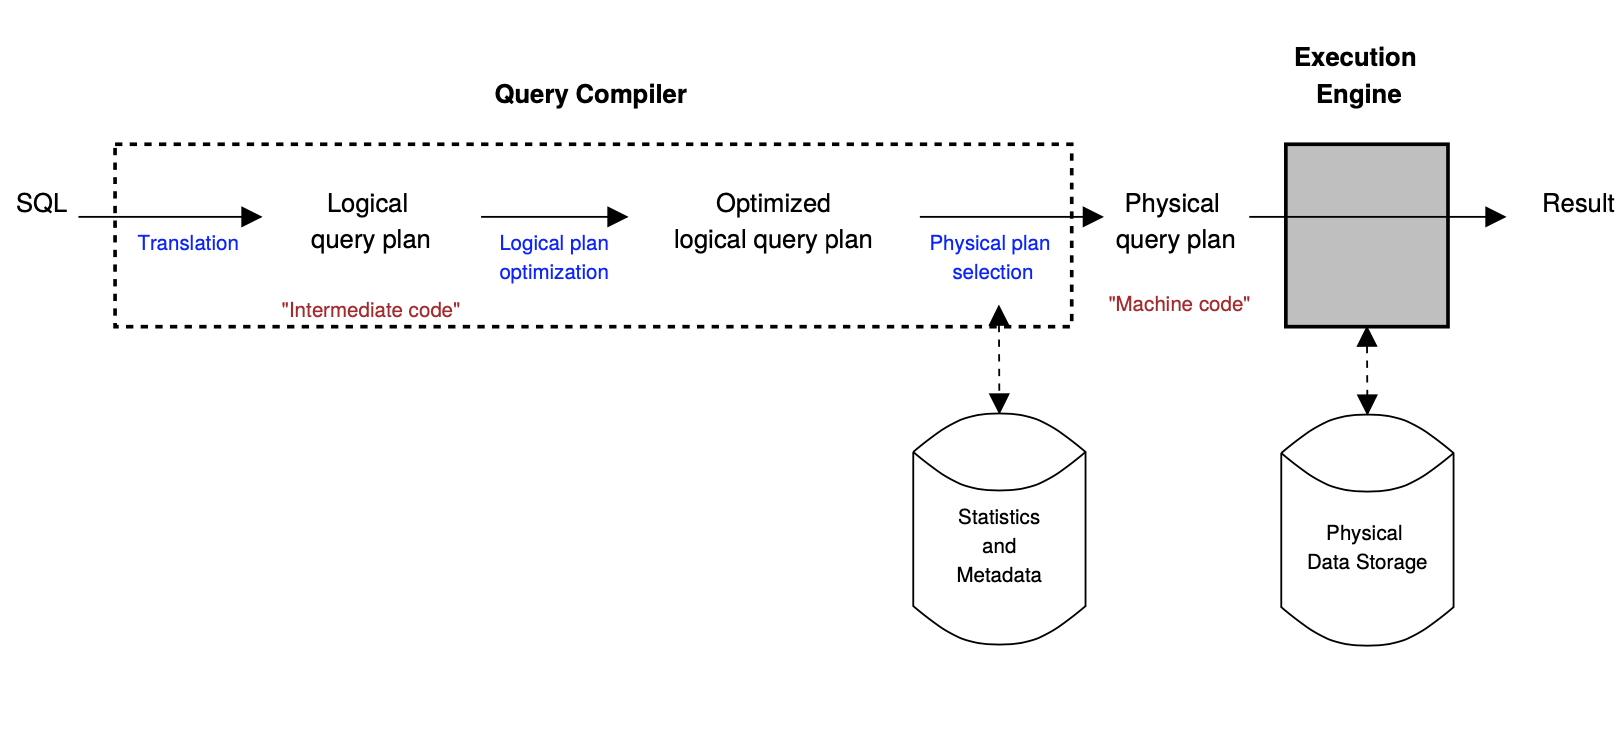
\includegraphics[scale=0.38]{img/img1.png}
	\captionof{figure}{Query Compiler}
\end{center}
At the "logical plan optimization" step, redundency are removed.
The "physical plan selection" tell \textit{how} we will proceed e.g. join those tables then do this sequential search. rmq : this is not the compilation in machine language, that's the compiler's job ! \\

Here we're interested in SQL text to logical to query plan part of the process.

\begin{center}
	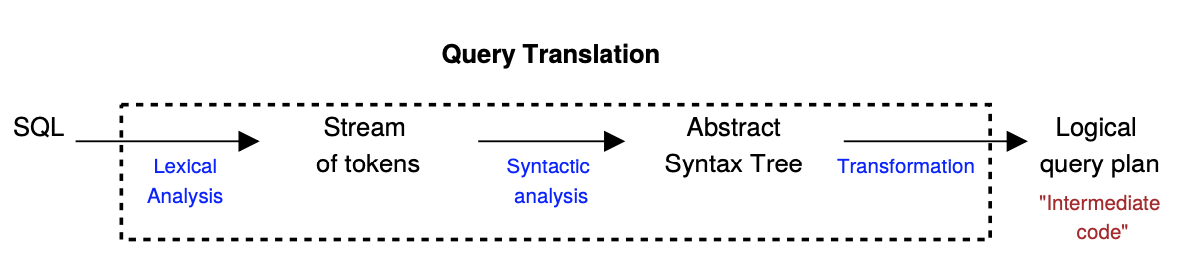
\includegraphics[scale=0.42]{img/img2.png}
	\captionof{figure}{Query Translation}
\end{center}

Simplifying assumption :
\begin{itemize}
\item only translate SQL-92 queries $\rightarrow$ basic instruction like SELECT, FROM, WHERE, GROUP BY, ...
\item set-based semantic meaning there is no \textbf{duplicate tuples}, otherwise it's bag-based (relation are usually bag-based)
\end{itemize}

\subsection{Memo on relational Algebra}
\textcolor{magenta}{Relation} are tables whose columns are called \textcolor{magenta}{attributes}. The set of all attributes of a relation is called the \textcolor{magenta}{schema} of the relation. The rows are called \textcolor{magenta}{tuple}.\\
Each Relational Algebra operator takes as input 1 or more relations, and produces a new relation.

\paragraph{Basic operation between table}

\begin{center}
	\begin{tabular}{c|c|c}
	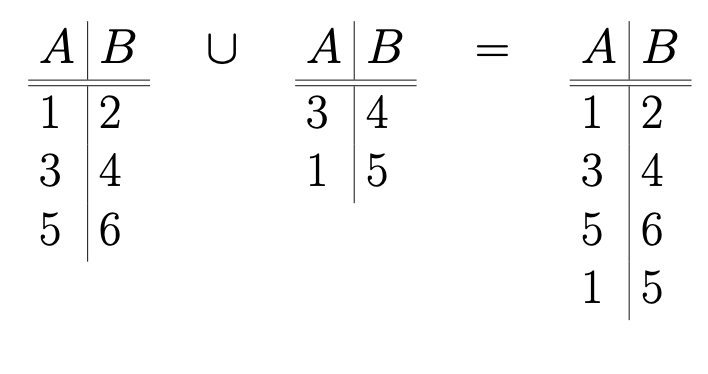
\includegraphics[scale=0.37]{img/img3.png}&
	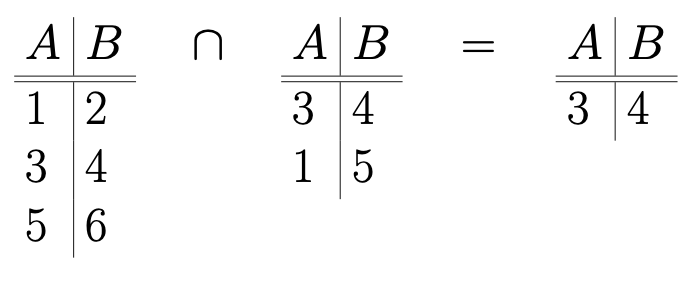
\includegraphics[scale=0.46]{img/img4.png}&
	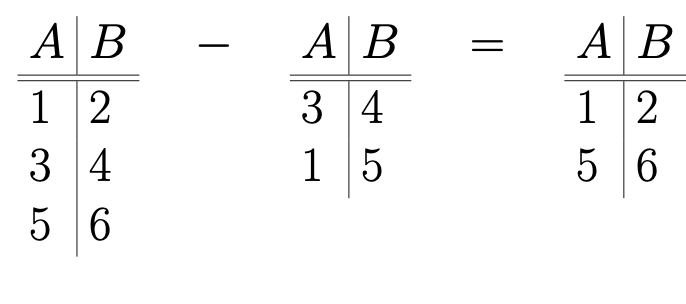
\includegraphics[scale=0.46]{img/img5.png}\\
\end{tabular}
	\captionof{figure}{Union (left), Intersection (center) and Difference (right)}
\end{center}

Input relations must have the same schema.\\

\paragraph{Basic operation on a table}
\begin{center}
\begin{tabular}{c|c}
	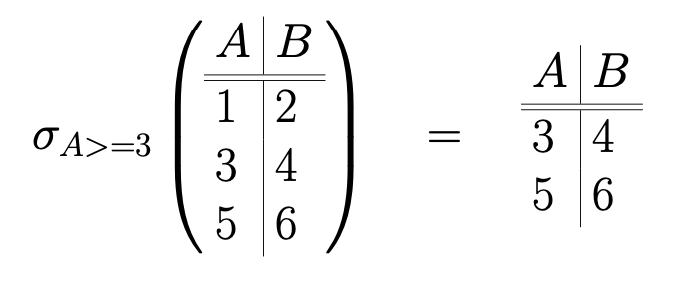
\includegraphics[scale=0.45]{img/img6.png}&
	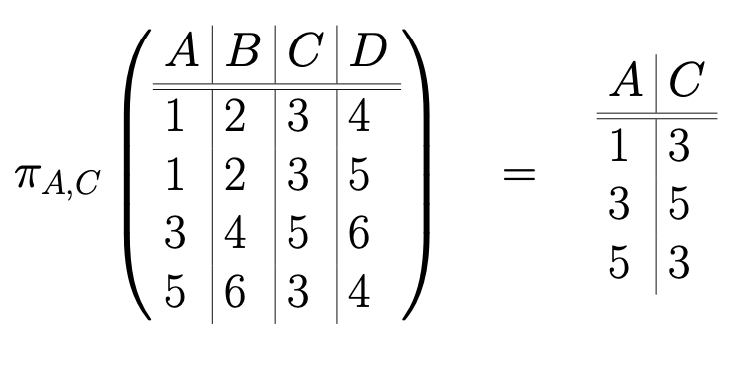
\includegraphics[scale=0.37]{img/img7.png}
\end{tabular}
	\captionof{figure}{Selection (left) and Projection (right)}
\end{center}
Here an ill formed selection would be a selection on an inexistant attribute. Since the projection is set-based we don't have twice the tuple (1,3).

\paragraph{Cartesian product}
\begin{center}
	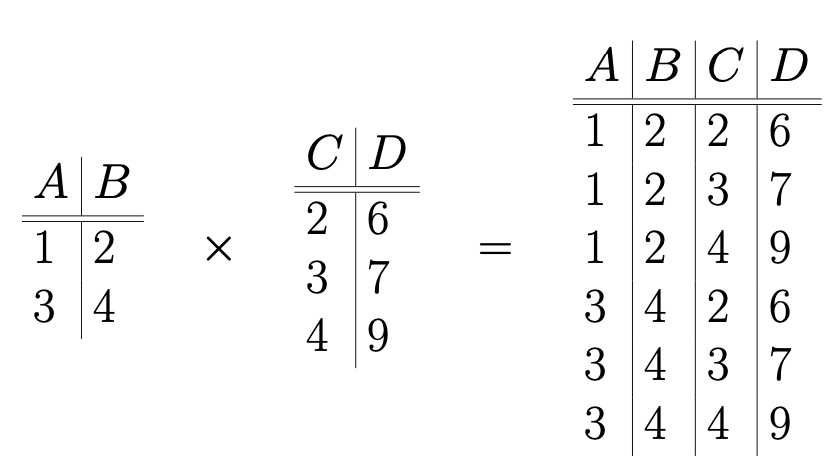
\includegraphics[scale=0.45]{img/img8.png}
	\captionof{figure}{Cartesian Product}
\end{center}

Input relations must have disjoint schema.

\paragraph{Join}
\begin{center}
\begin{tabular}{c|c}
	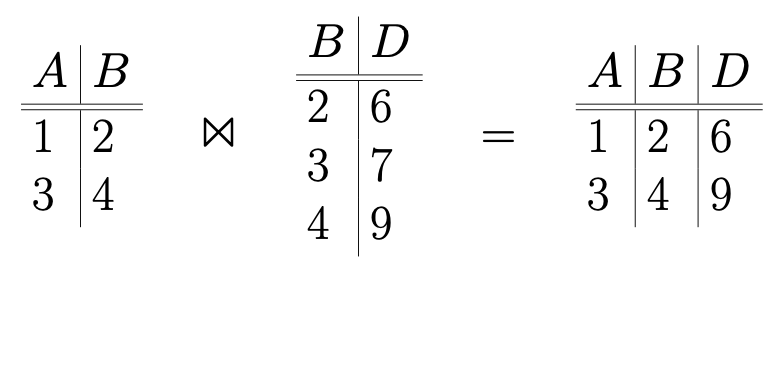
\includegraphics[scale=0.41]{img/img9.png}&
	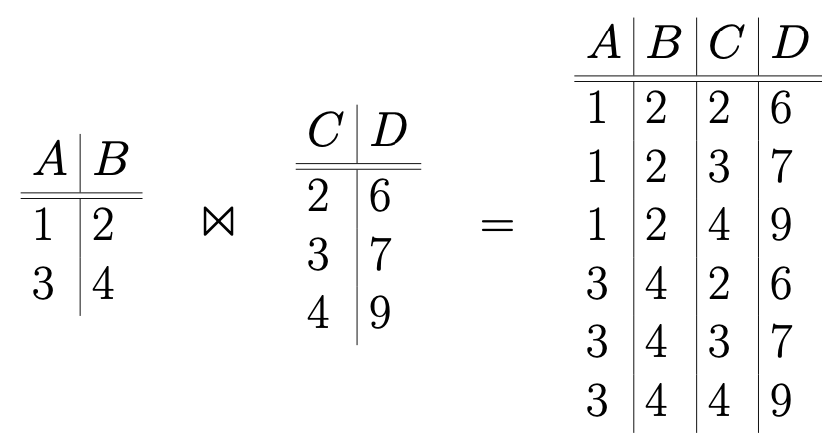
\includegraphics[scale=0.42]{img/img10.png}\\
	\hline
\end{tabular}
	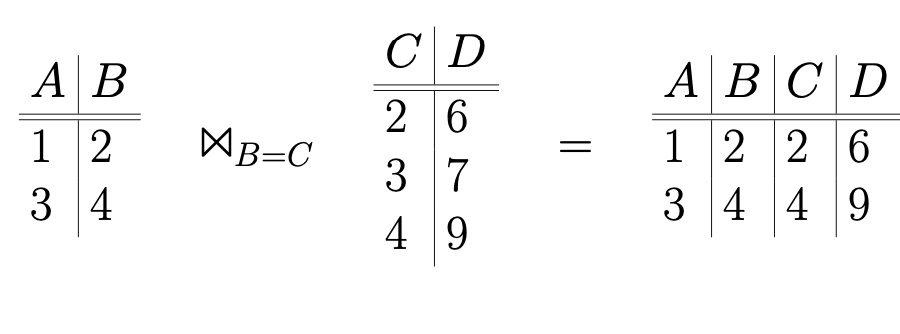
\includegraphics[scale=0.40]{img/img11.png}
	\captionof{figure}{Natural Join with common attribute (upper left), Natural Join without common attribute (upper right) and Theta Join (bottom)}
\end{center}
Join occurs when there are identical value for the common attribute.\\
A Natural Join without common attribute occurs like a Cartesian Product.\\
The antijoin operator also exist :
$R \antijoin S \equiv R - (R \Join S)$

\paragraph{Renaming}
 \begin{center}
	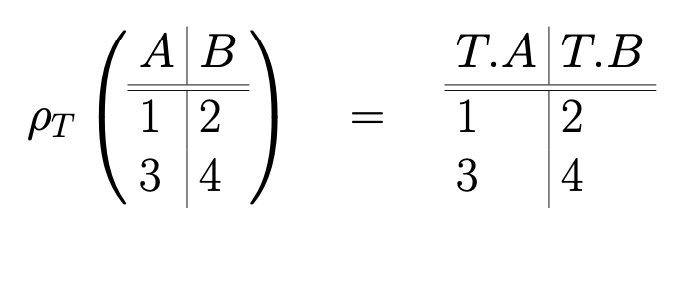
\includegraphics[scale=0.45]{img/img12.png}
	\captionof{figure}{Renaming}
\end{center}
Renaming specifies that the input relation (and its attributes) should be given a new name.

\paragraph{Extented relational algebra - Grouping}
\begin{center}
	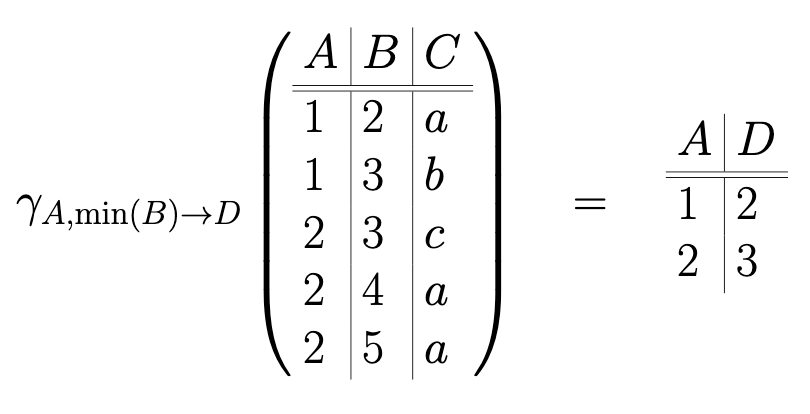
\includegraphics[scale=0.45]{img/img13.png}
	\captionof{figure}{Grouping}
\end{center}
One of the more important operator of \emph{extended} relational algebra. We group by attribute A then take the minimum B of each group. Grouping on multiple attribute is also possible.

\paragraph{Extented relational algebra - Extended Projection}
\begin{center}
	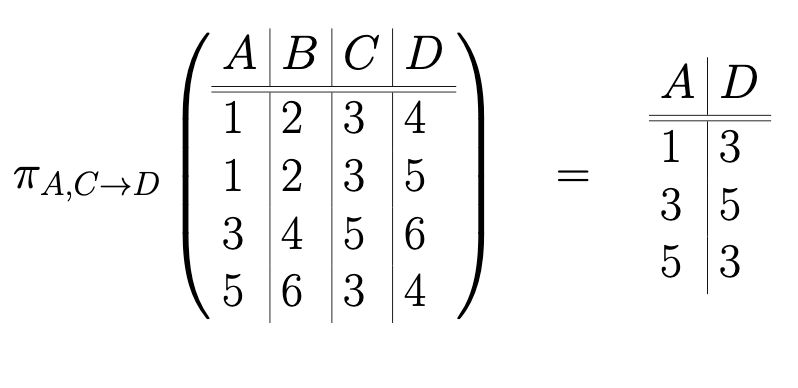
\includegraphics[scale=0.45]{img/img14.png}
	\captionof{figure}{Projection}
\end{center}
Like the projection we but also rename one of the colone

\paragraph{Expression}
$$\sigma_{\text{length}\geq 100}(\text{Movie}) \Join_{\text{title}=\text{movietitle}} \text{StarsIn} $$
They are built using relation variable and relational algebra operator. It says what we compute but not how (eg should we use an index, parcours the entirety of the table, ...).

\paragraph{Sets and Bags}
All previous operator were sets based - without duplicates tuple. In practice allowing duplicates is more efficient $\rightarrow$ bags based relations. This imply that some operator changes, for exemple
\begin{center}
	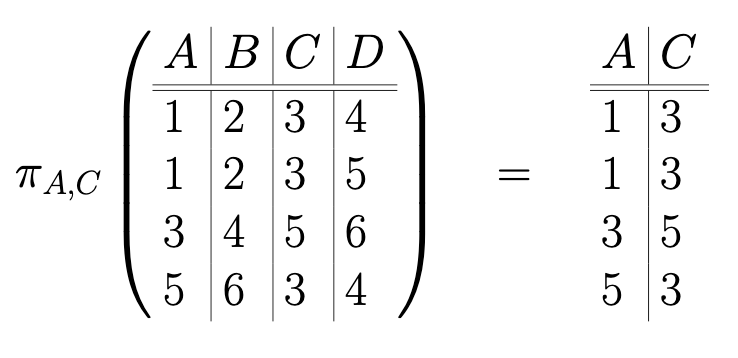
\includegraphics[scale=0.45]{img/img15.png}
	\captionof{figure}{bag-based projection}
\end{center}
The modified operators are Union, Intersection, Difference and Projection. The other are simply straightforwardly extended.

\subsection{translating select-from-where}
Simple "select-from-where" queries without subqueries is pretty straightforward.
\begin{verbatim}
SELECT movieTitle
FROM StarsIn, MovieStar M
WHERE starName = M.name AND M.birthdate = 1960
\end{verbatim}
The select becomes the projection, the from gives the table for the cartesian product and the where gives the selection :
$$\pi_{\text{movieTitle}}\sigma_{\text{starName}=\text{M.name}\bigwedge \text{M.birthdate}=1960}(\text{StarsIn} \times \rho_M (\text{MovieStar})$$

Subqueries occurs through the operators $=,<,>,\leqslant, \geqslant, <>$; through quantifiers ANY, ALL; through operator EXISTS, IN, NOT EXISTS, NOT IN.\\
All subqueries can be normalized into only EXISTS or NOT EXISTS as showed below.
\begin{center}
	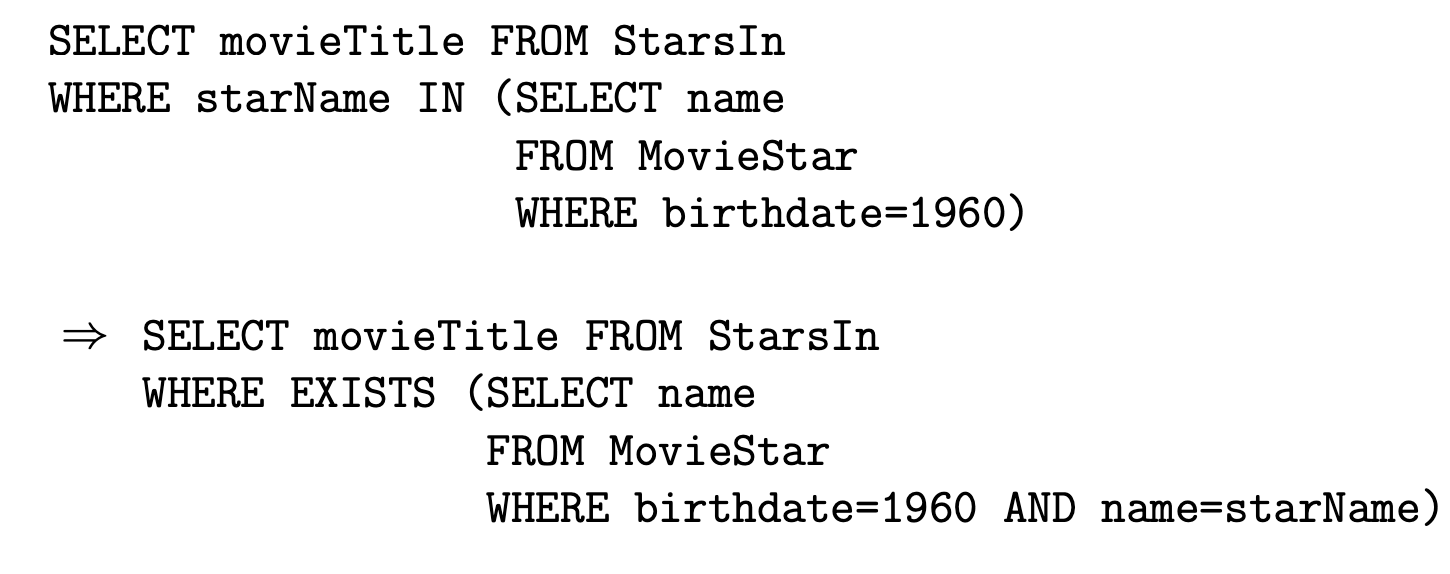
\includegraphics[scale=0.4]{img/img16.png}
	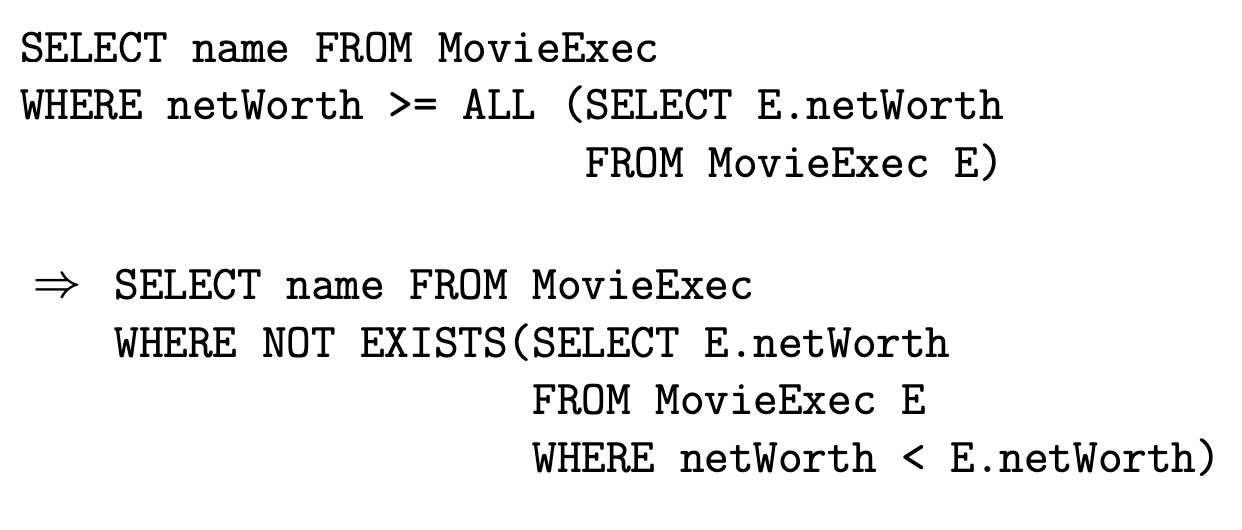
\includegraphics[scale=0.4]{img/img17.png}
	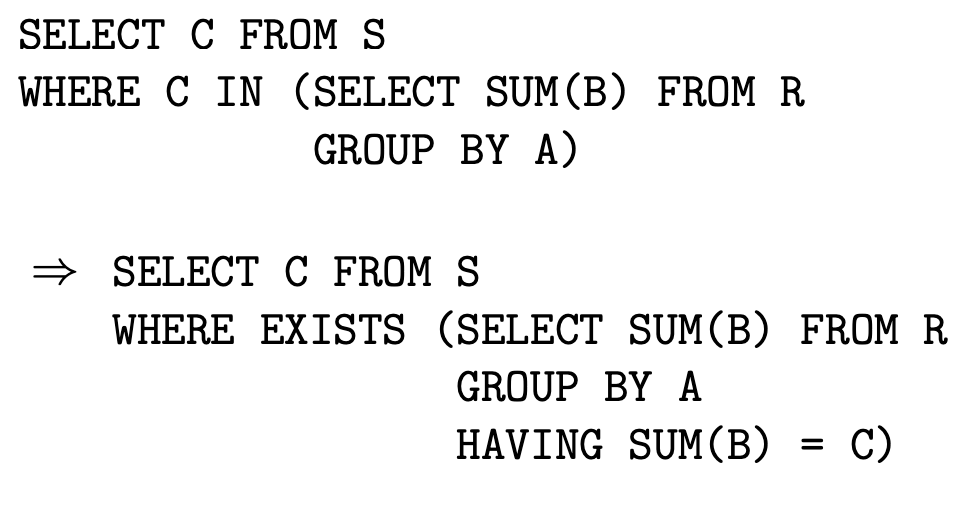
\includegraphics[scale=0.4]{img/img18.png}
	\captionof{figure}{Normalization of subqueries}
\end{center}

Our normalized subqueries can refer to attribut of relation that are introduced in the outer query, those subqueries are called \emph{correlated subqueries}. The other relation used in the subquery are called \emph{context relations}, the attribute of all context relation are the \emph{parameters} of the subquery.\\

Exemple of translating a correlated s-f-w subquery :
\begin{verbatim}
SELECT S.movieTitle, M.studioName 
FROM StarsIn S, Movie M 
WHERE S.movieYear >= 2000
AND S.movieTitle = M.title
AND EXISTS (SELECT name
            FROM MovieStar
			WHERE birthdate=1960 AND name= S.starName)
\end{verbatim}

\begin{enumerate}
\item translate EXIST subquery : $\pi_{\text{name}} \sigma_{\text{birthdate}=1960 \bigwedge \text{name=S.starName}} (\text{MovieStar}) $
\item add \textcolor{red}{context relation} and \textcolor{blue}{parameter} : $$\pi_{\text{\textcolor{blue}{S.movieTitle,S.movieYear,S.starName},name}} \sigma_{\text{birthdate}=1960 \bigwedge \text{name=S.starName}} (\text{MovieStar} \textcolor{red}{\times \rho_S(\text{StarsIn})}) $$
\item translate FROM clause of the outer query : $\rho_S(\text{StarsIn}) \times \rho_M(\text{Movie})$
\item synchronised the sub result with a join :
$$(\rho_S(\text{StarsIn}) \times \rho_M(\text{Movie})) \Join$$
$$\pi_{\text{S.movieTitle,S.movieYear,S.starName,name}} \sigma_{\text{birthdate}=1960 \bigwedge \text{name=S.starName}} (\text{MovieStar} \times \rho_S(\text{StarsIn}))$$
\item simplify by omitting the first StarsIn, the parameters are already there thanks to the subquery :
$$\rho_M(\text{Movie}) \Join$$
$$\pi_{\text{S.movieTitle,S.movieYear,S.starName,name}} \sigma_{\text{birthdate}=1960 \bigwedge \text{name=S.starName}} (\text{MovieStar} \times \rho_S(\text{StarsIn}))$$
\item Translate the WHERE and SELECT clause from the outer query :
$$\pi_{\text{S.movieTitle,M.studioName}}\sigma_{\text{S.movieYear}\geqslant1960 \bigwedge \text{S.movieTitle=M.title}}$$
$$(\rho_M(\text{Movie}) \Join \pi_{\text{S.movieTitle,S.movieYear,S.starName,name}}$$
$$\sigma_{\text{birthdate}=1960 \bigwedge \text{name=S.starName}} (\text{MovieStar} \times \rho_S(\text{StarsIn})))$$
\end{enumerate}
If the subquery is an NOT EXISTS the process is the same execept that the synchronization at point 4 is done with an antijoin $\antijoin$ and the simplification at point 5 is impossible since we need the tuple that are StarsIn but not in the subquery.\\

To treat a query of the form :
\begin{verbatim}
SELECT Select-list FROM From-list 
WHERE A=B AND NOT(EXISTS(Q) AND C<6)
\end{verbatim}
We first transform it into :
\begin{verbatim}
SELECT Select-list FROM From-list
WHERE (A=B AND NOT EXISTS(Q)) OR (A=B AND C>=6)
\end{verbatim}
Then use morgan's law on the OR and obtain :
\begin{verbatim}
(SELECT Select-list FROM From-list 
WHERE (A=B AND NOT EXISTS(Q))) 
UNION
(SELECT Select-list FROM From-list 
WHERE (A=B AND C>=6))
\end{verbatim}
They are more exemple or case like this in the last 10 slides of lect1. It's not very interessting to just copy them all here.

\section{Optimization of Logical Query Plans - lecture 2}
Now that we have the logical query plan, we need to optimized it ! A logical query plan $\pi_{A,B}(\sigma_{A=5}(R)\cup(S \Join T))$ is essentially an execution tree :
\begin{center}
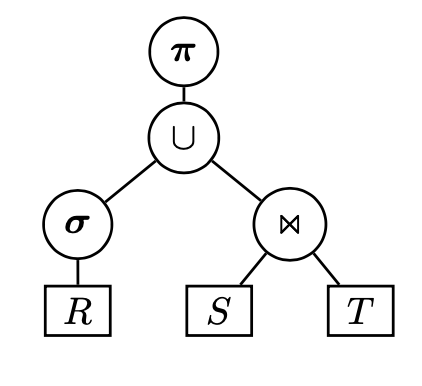
\includegraphics[scale=0.4]{img/img19.png}
\captionof{figure}{execution tree}
\end{center}
It is sometimes possible to simplify those execution tree by removing some nodes and still obtains the same result but faster. Rmq : a physical query plan is a logical query plan where each node is assigned an algorithm $\rightarrow$ done in section 5 and 6.\\
\textbf{Definition :} A relational algebra expression $e$ is optimal if there is no other expression $e'$ that is both (1) equivalent to $e$ and (2) “shorter” than $e$ (i.e., has fewer occurrence of operators than $e$).\\
Meaning the optimization problem takes as input $e$ and outputs a $e'$.
The optimization problem is undecidable, proof is done by showing that a decidable optimization problem imply that another problem - known undecidable - is in fact decidable. (preuve par l'absurde en gros)\\
However we can still optimize that using the form select-project-join.

\paragraph{select-project-join}
$$\pi_{...}\sigma_{A_1=B_1 \wedge A_2=B_2 \wedge ... \wedge A_n = B_n}(R_1 \times R_2 \times ... \times R_m)$$
select-project-join are expression where we only use relation, renaming, projection, selection, equality and join (so no union, $-, \neq,<$,...). Joins are the most costly operations so if we can remove some it would be nice.\\

\paragraph{Conjuctive query}
By definition it is an expression of the form : 
$$Q\underbrace{(x_1,...,x_n)}_{\text{head}}\leftarrow \underbrace{R(t_1,...,t_m),...,S(t_1',...,t'_k)}_{\text{body}}$$
Here $t_1, . . . , t'_k$ denote variables and constants, and $x_1, . . . , x_n$ must be variables that occur in $t_1,...,t'_k$. We call an expression like $R(t_1,...,t_m)$ an atom. If an atom does not contain any variables, and hence consists solely of constants, then it is called a fact.\\

Example : 
\begin{center}
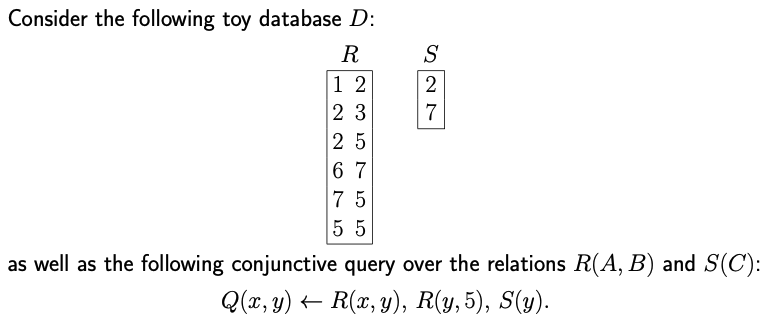
\includegraphics[scale=0.4]{img/img20.png}
\end{center}
Intuitively, $Q$ wants to retrieve all pairs of values $(x,y)$ such that (1) this pair occurs in relation $R$; (2) $y$ occurs together with the constant 5 in a tuple in $R$; and (3) $y$ occurs as a value in $S$. The formal definition is as follows : a subsitution $f$ of $Q$ into $D$ is a function that maps variable in $Q$ to constants in $D$. For example $f : x \mapsto 1, y \mapsto 2$\\
A matching is a substitution that maps the body of $Q$ into facts in $D$. For example: $f : x \mapsto 1, y \mapsto 2$\\
The result of the query are the variable that can be assigned to $x$ and $y$ in such way that $R(x,y)$, $R(y,5)$ and $S(y)$ are in $D$. Or more formally : The result of a conjunctive query is obtained by applying all possible matchings to the head of the query. In our example: $Q(D) = \lbrace(1,2),(6,7)\rbrace$\\
The optimization will be done on the conjunctive query meaning we have to translate the select-project-join expression into a conjunctive query :
\begin{center}
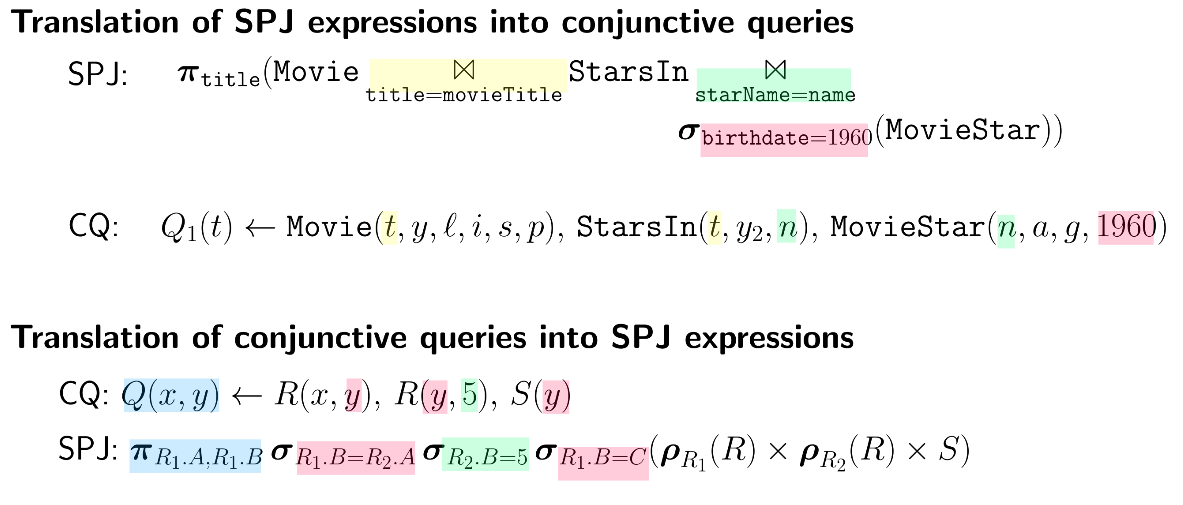
\includegraphics[scale=0.3]{img/img21.png}
\end{center}

\paragraph{Containement of conjunctive queries}
$Q_1$ is contained in $Q_2$ if $Q_1(D) \subseteq Q_2(D)$, for every database $D$, meaning that every solution of $Q_1$ is also a solution of $Q_2$. It's the case whenever $Q_1$ has more strict condition than $Q_2$. (Detail of the methology with cannonical database at the end.)\\
We try to simplify the expression $Q$ by removing an atom, if the new expression $Q_1$ gives us $Q \subseteq Q_1$ and $Q_1 \subseteq Q$ then the 2 expression are equivalent and we can keep $Q_1$ as the new expression.\\
\\
Once $Q$ has been simplified, we translate it back to select-project-join expression and we can try to use heuristic to further optimize it :
\begin{center}
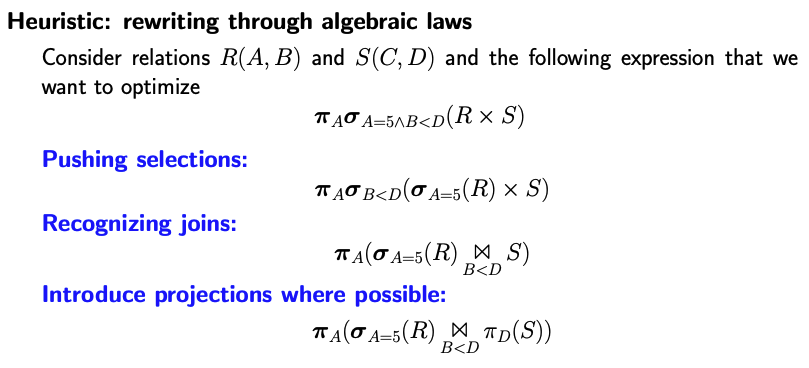
\includegraphics[scale=0.4]{img/img22.png}
\end{center}

\section{Physical data organisation}
This part was a reading assignement.

\section{Index Structure}
Data is stored on disk divided into blocks of bytes. The CPU can only work on data item stored in memory an not directly on the disk. So data must be transfered from the disk to memory in whole block at the time. This transfer is the \textbf{more costly} part ! Capacity of the memory is far inferior to the capacity of the disk. The execution time and thus the cost are dominated by the disk I/O. The number of I/O is gonna be used as the cost metric for operation.\\
If we want to look for tuple with a certain value for an attribute; we can charge in memory each block and search inside but it's gonna be very long ! Main objectif of Index Structure is to reduce the number of I/O needed.

\subsection{One-dimensional Index Strutcure - lecture 3}
\textbf{Definition :} An index structure is any data structure that takes as input a search key and \emph{efficiently} returns the collection of matching records.\\

\subsubsection{Conventional Indexes}
Our index can be either \emph{dense} or \emph{sparse} and can be on a \emph{primary} or \emph{secondary} key. First let's assume that the search key will be the primary key and our data is already sorted on that first key. The index will contain the value of the key and the address of the record with this value in the sequential file. We assume we can store 4 pairs (key, pointer) per block for the index. Now we can have a record with each value of the key - dense index - or only some of those values - sparse index - we onlty stock value of the key at the begining of a block in the sequential file.
\begin{center}
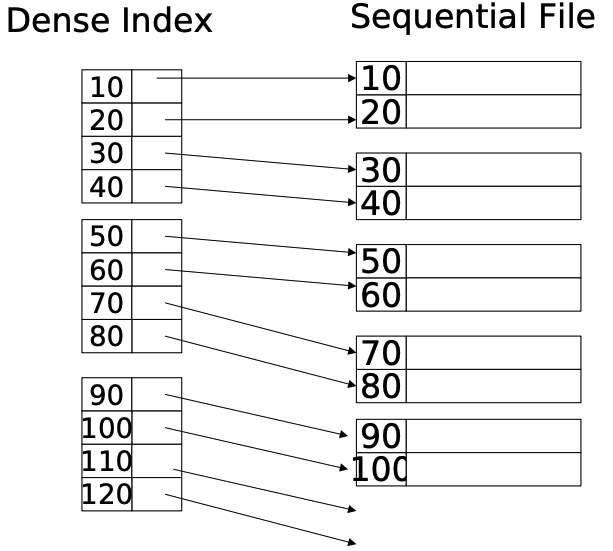
\includegraphics[scale=0.3]{img/img23.png}
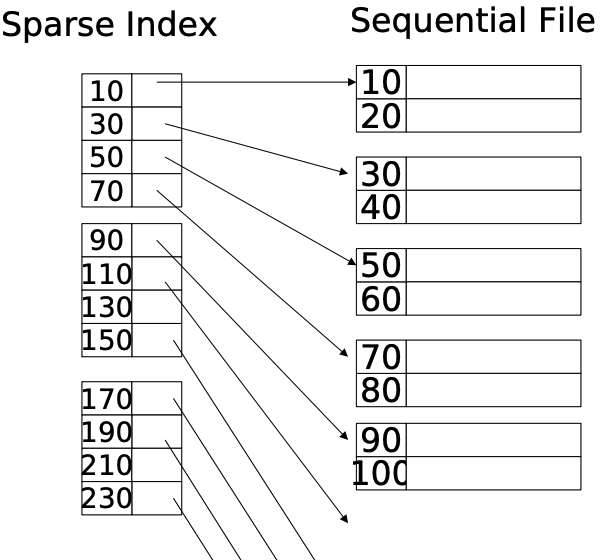
\includegraphics[scale=0.3]{img/img24.png}
\captionof{figure}{Dense index (left) and Sparse Index (right)}
\end{center}
In both case the index is smaller than the sequential file and thus necessite less I/O to read. But where the dense index is half the length of the seq file, the sparse index is a quarter of the initial size ! And for additional speed we can even add a second level sparse index.
\begin{center}
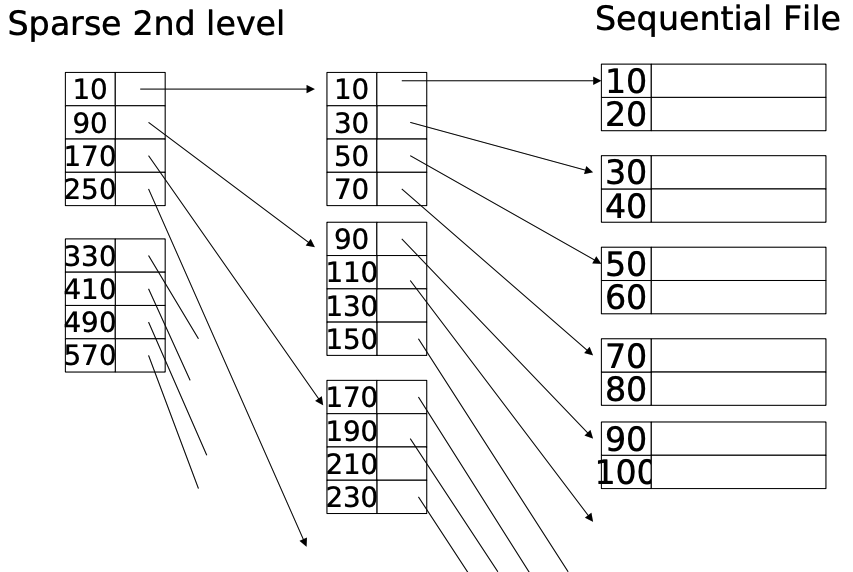
\includegraphics[scale=0.34]{img/img25.png}
\end{center}
If we want to find the record where key = 45, we load block in the 2nd level index for 10, then load block in the 1st level for 30 then go to 45. The more level we add the smaller in size each additional level. The worst case scenario is having to do a linear search on the outmost level.
However this system cause problems when we want to add or delete record ...
(Doing a 2nd dense level would be pointless, it doesn't reduce the length). The advantage of the dense index is that we can see if a record exist without accessing the sequential file.

\paragraph{Duplicate keys}
What happens when a search key appears multiple times ? For dense index we can either have one record for each occurence of the key or just one record for the first occurene of the key. For sparse index we can have a record for each key at the beginning of a block (left below) or store the value of the first new key for each address of a block (right below).
\begin{center}
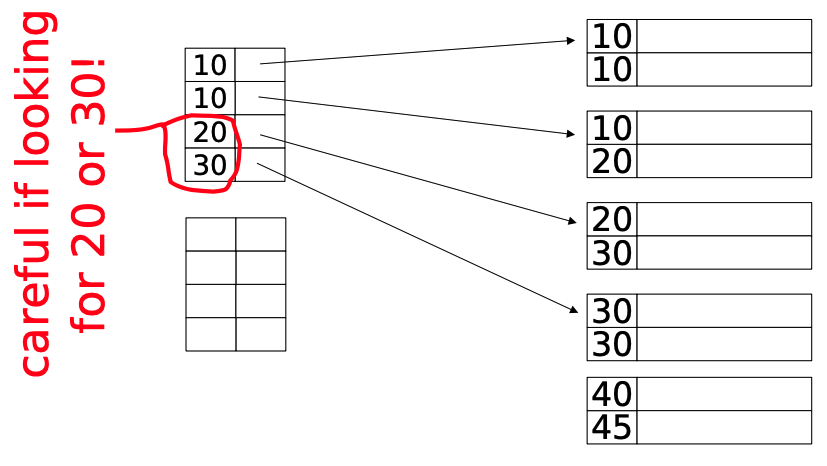
\includegraphics[scale=0.25]{img/img26.png}
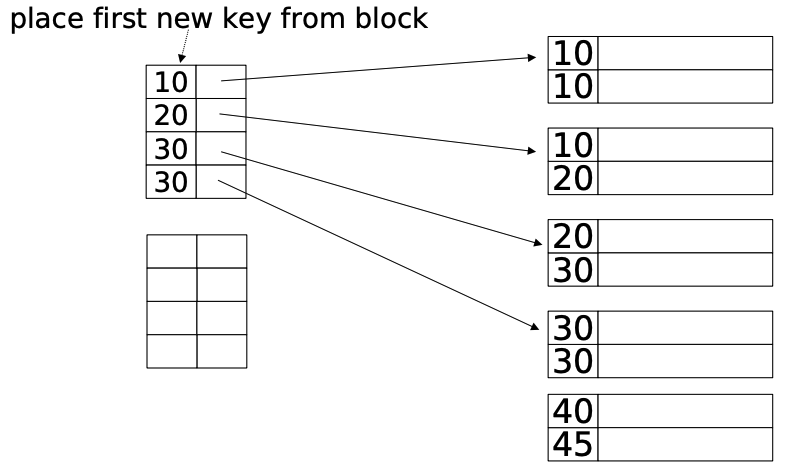
\includegraphics[scale=0.25]{img/img27.png}
\end{center}


\paragraph{Deletion/Insertion}
We consider a case where there is maximum one on each key.
To delete in a sparse index, we first have to find where the record is located by using the index. then we can remove the record and see if we have to change the index. If we remove record 40 it doesn't change the index but if we remove record 30 then 40 become the first record in the block and the index must be updated. If we remove both 30 and 40 then the index changes a lot and we have to move the block for 50 and 70 up. 
\begin{center}
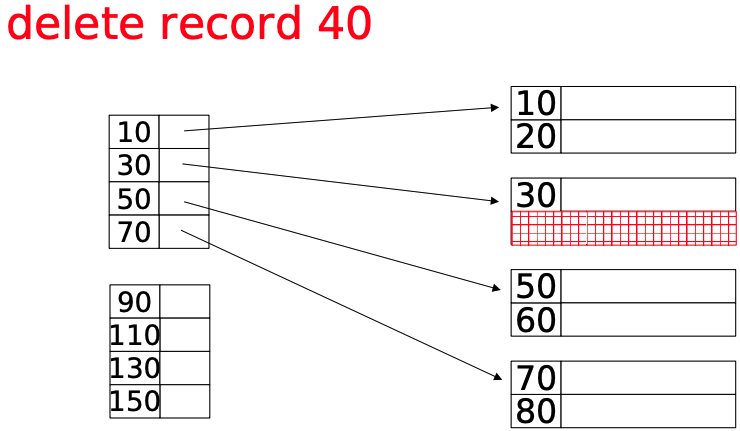
\includegraphics[scale=0.2]{img/img28.png}
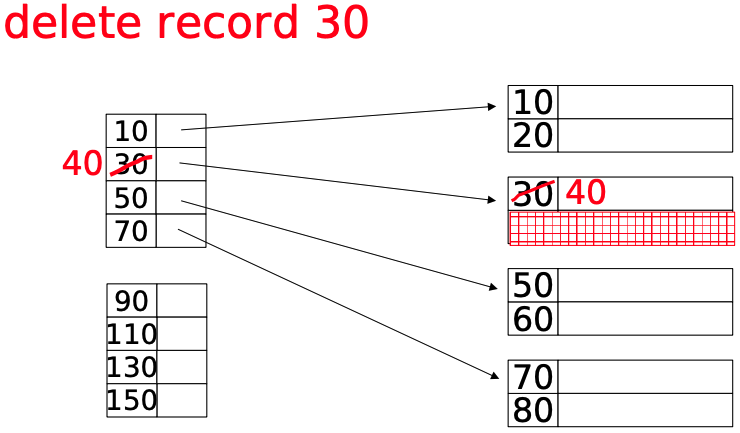
\includegraphics[scale=0.2]{img/img29.png}
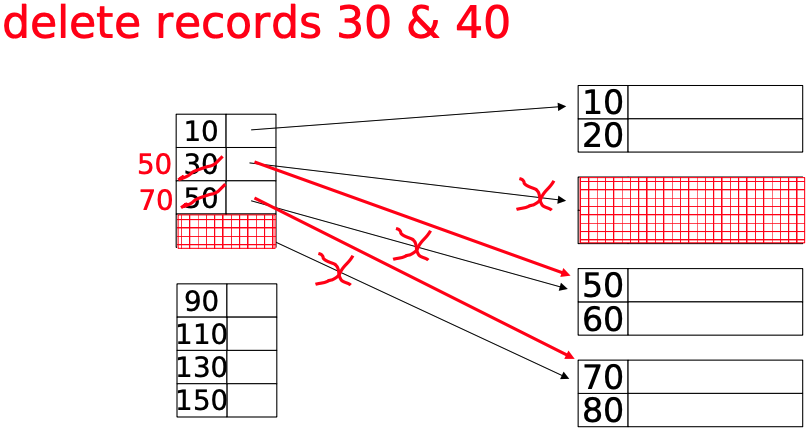
\includegraphics[scale=0.2]{img/img30.png}
\end{center}

When we deleted record with a dense index, the index must be updated each time.\\

For insertion in a sparse index, if there is a available slot in the sequential file then we are lucky and can insert immediatly the new record. Else we have to shift The record untill there is an empty space. The index must also be updated. If we're unlucky then we have to shift the entire database. \\
A way to circumvent this is to insert new block in chained file. However if the overflow line become too big then the cost of a search can become linear. Usually we only reorganise the databise once we reach a threshold in the overflow length.
\begin{center}
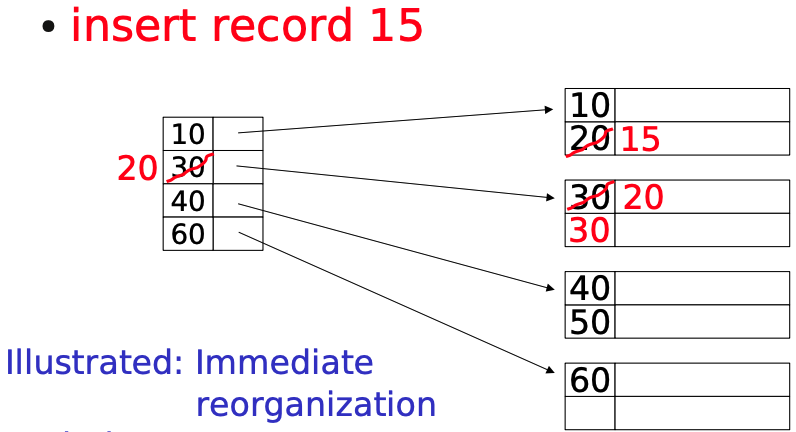
\includegraphics[scale=0.25]{img/img31.png}
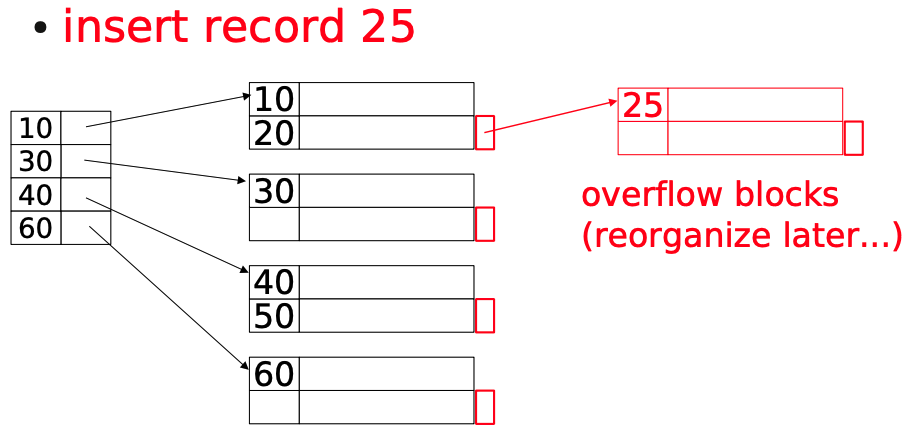
\includegraphics[scale=0.25]{img/img32.png}
\end{center}
The process is similar for dense index and often more expensive.

\paragraph{Secondary indexes}
Sometimes our search key is in fact a secondary indexes, meaning the records aren't in order. Doing a sparse index as done before (first block) would not make sense. We first haev to build a (sorted) dense index before a sparse one can be build. (Also the pointers are record pointers and not block pointers)
\begin{center}
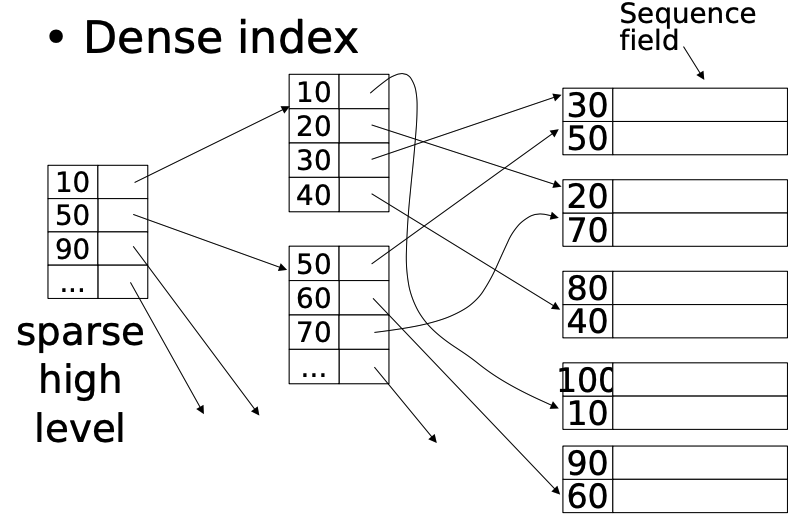
\includegraphics[scale=0.3]{img/img33.png}
\end{center}

When they are duplicate value combined with secondary index, the best idea is to use intermediates bucket. The bucket is a separate file stocking the pointers toward the database. They are also usefull for query on more than one index.
\begin{center}
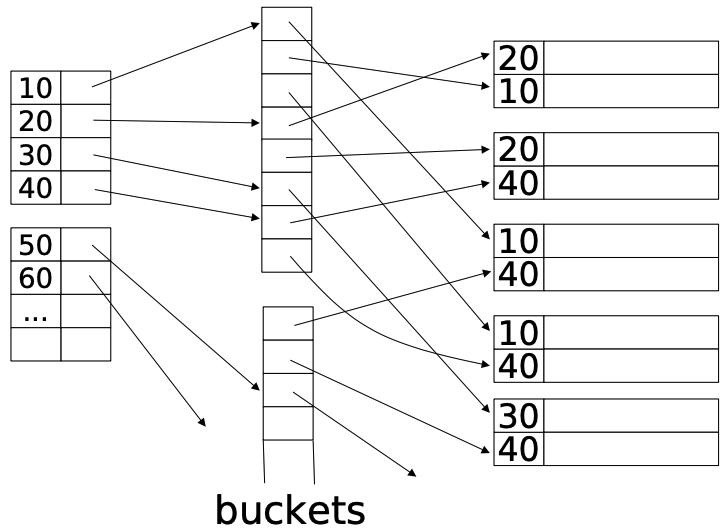
\includegraphics[scale=0.28]{img/img34.png}
\end{center}

\subsubsection{B trees}
\begin{wrapfigure}[11]{r}{8.1cm}
\vspace{-5mm}
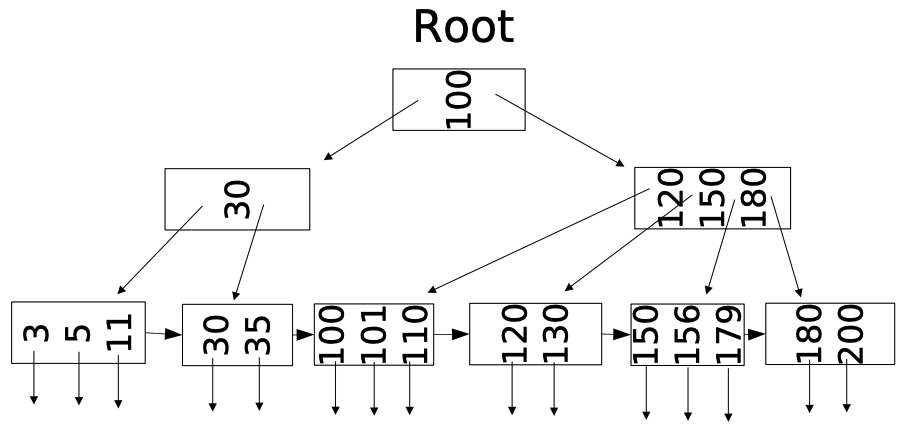
\includegraphics[scale=0.27]{img/img35.png}
\captionof{figure}{Example of a B-Tree, n = 3}
\end{wrapfigure}

While conventional indexes are simple and good for scan, the insert are expensive and/or lose sequentiality and balance. B-tree indexes don't try to achieve sequentiality of the index but focus on the "balance".\\
They are one of the most used index system. A B-Tree is composed of nodes, the ones at the bottom are the leaf.\\
The non-leaf node $120-150-180$ has pointers toward keysmaller than 120, between 120 and 150, between 150 and 180 and over 180. The leaf node $150-156-179$ has pointers toward record with key 150, 156 and 179 and also a pointer to the next leaf in sequence. Nodes all have a fixed size of $n+1$ pointers and $n$ keys. Here is another notation :
\begin{center}
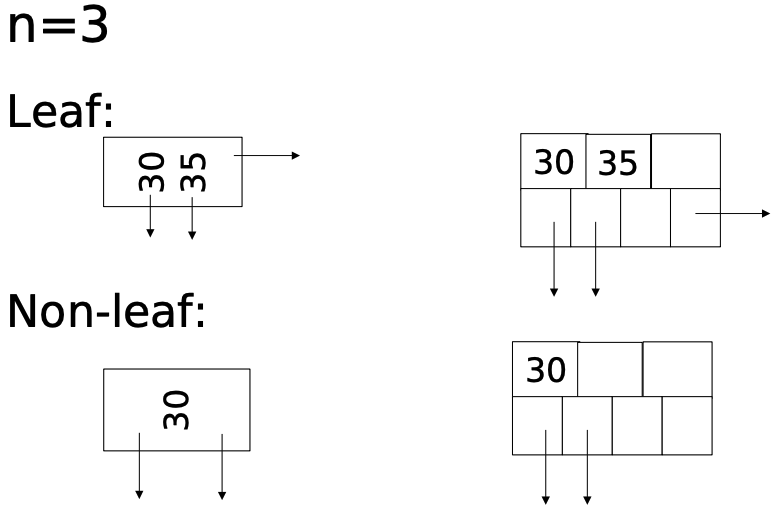
\includegraphics[scale=0.2]{img/img36.png}
\end{center}
To search for a record, we begin at the root then check the "direction"  and follow the pointers untill we reach a leaf. B-Tree also allow us to do range query.\\
The I/O cost of a lookup in a BTree is equal to the longest path of the root to a leaf. The goal is then to keep this path as short as possible and in particular to have all leafs at the same deep $\rightarrow$ keeping a balanced tree.\\
\\
Rules of BTree :
\begin{enumerate}
\item All leaves at same lowest level
\item Pointers in leaves point to record except for "sequence pointer"
\item Number of pointers/key for BTree :\\
\begin{tabular}{c|c|c|c|c|}
&Max ptrs & Max keys & Min ptrs$\rightarrow$data & Min keys\\
\hline
Non-leaf (non-root)& $n+1$ & $n$ & $\lceil (n+1)/2 \rceil$ & $\lceil (n+1)/2 \rceil - 1$\\
\hline
Leaf (non-root)& $n+1$ & $n$ & $\lfloor (n+1)/2 \rfloor$ & $\lfloor (n+1)/2 \rfloor$\\
\hline
Root& $n+1$ & $n$ & 2 & 1\\
\hline
\end{tabular}
\end{enumerate}
The last rule is there because we don't want empty nodes.

\paragraph{Insert}
Insertion of a new record can be very easy if there is available space in the leaf (a) or it can requiert a leafoverflow (b), non-leaf overflow (c) or even a new root (d).\\
In situation (a), a new pointer can simply be added to the correct leaf since there is available space. The I/O cost of this insertion is the cost of the search to find the correct leaf + 1 to write the new block.\\

\begin{wrapfigure}[9]{l}{6.4cm}
\vspace{-5mm}
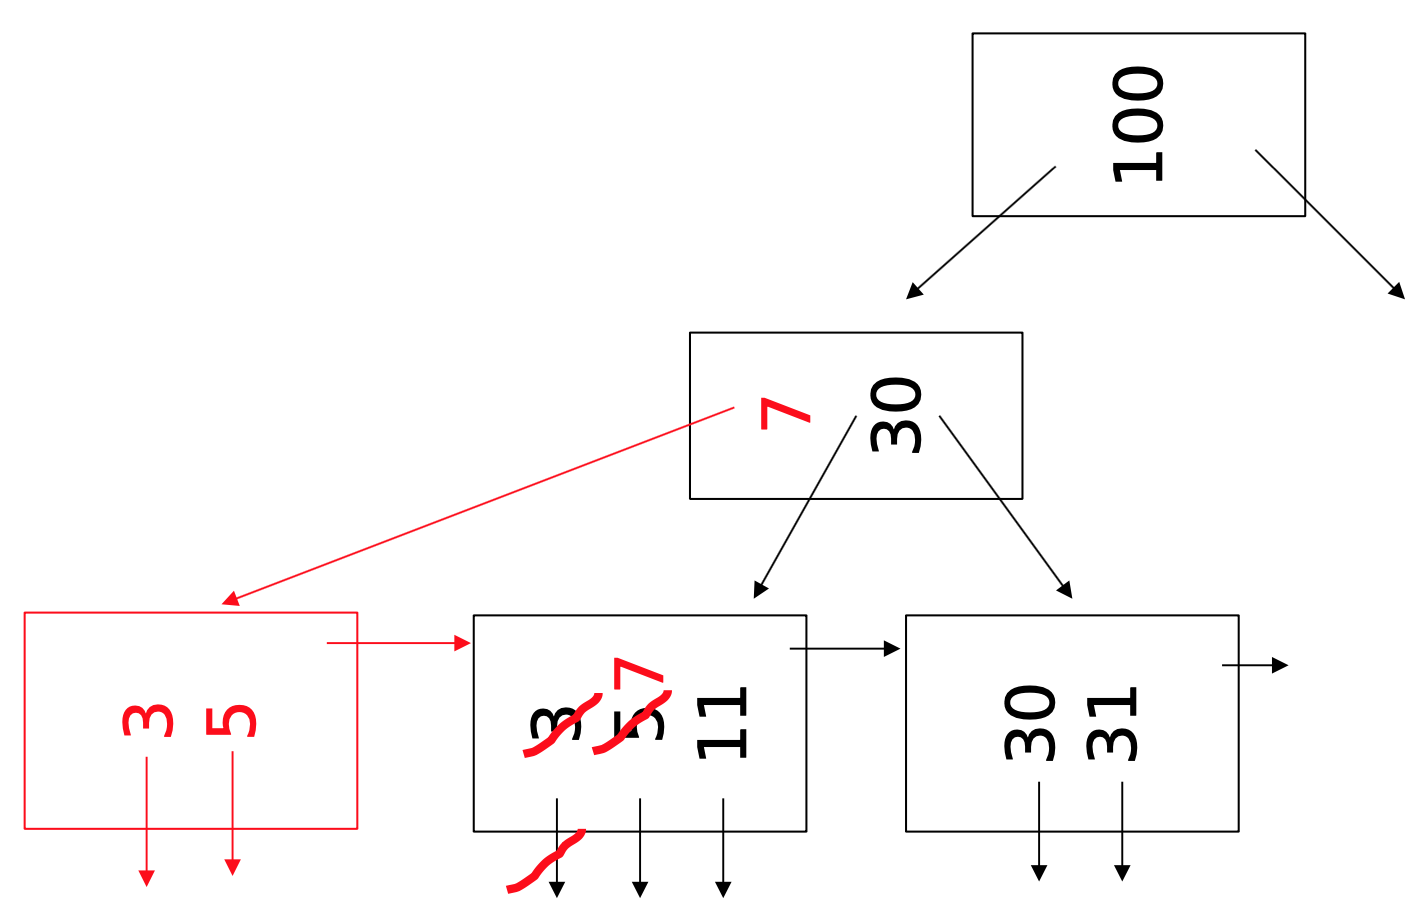
\includegraphics[scale=0.25]{img/img37.png}
\end{wrapfigure}
In scenario (b) there is no space in the leaf where we must insert. We will create a new leaf block and distribute the data such that both blocks are at least half-full (contains 2 pointer if n = 3). Because we rearange data, a new blocks is created and there must be pointer towards it. Also the minimum value in the existing block has changed. So the parent must be modified. Here the number of I/O is cost of searching + writing in 3 blocks (leafs + parents).\\

\begin{wrapfigure}[9]{r}{8.4cm}
\vspace{-5mm}
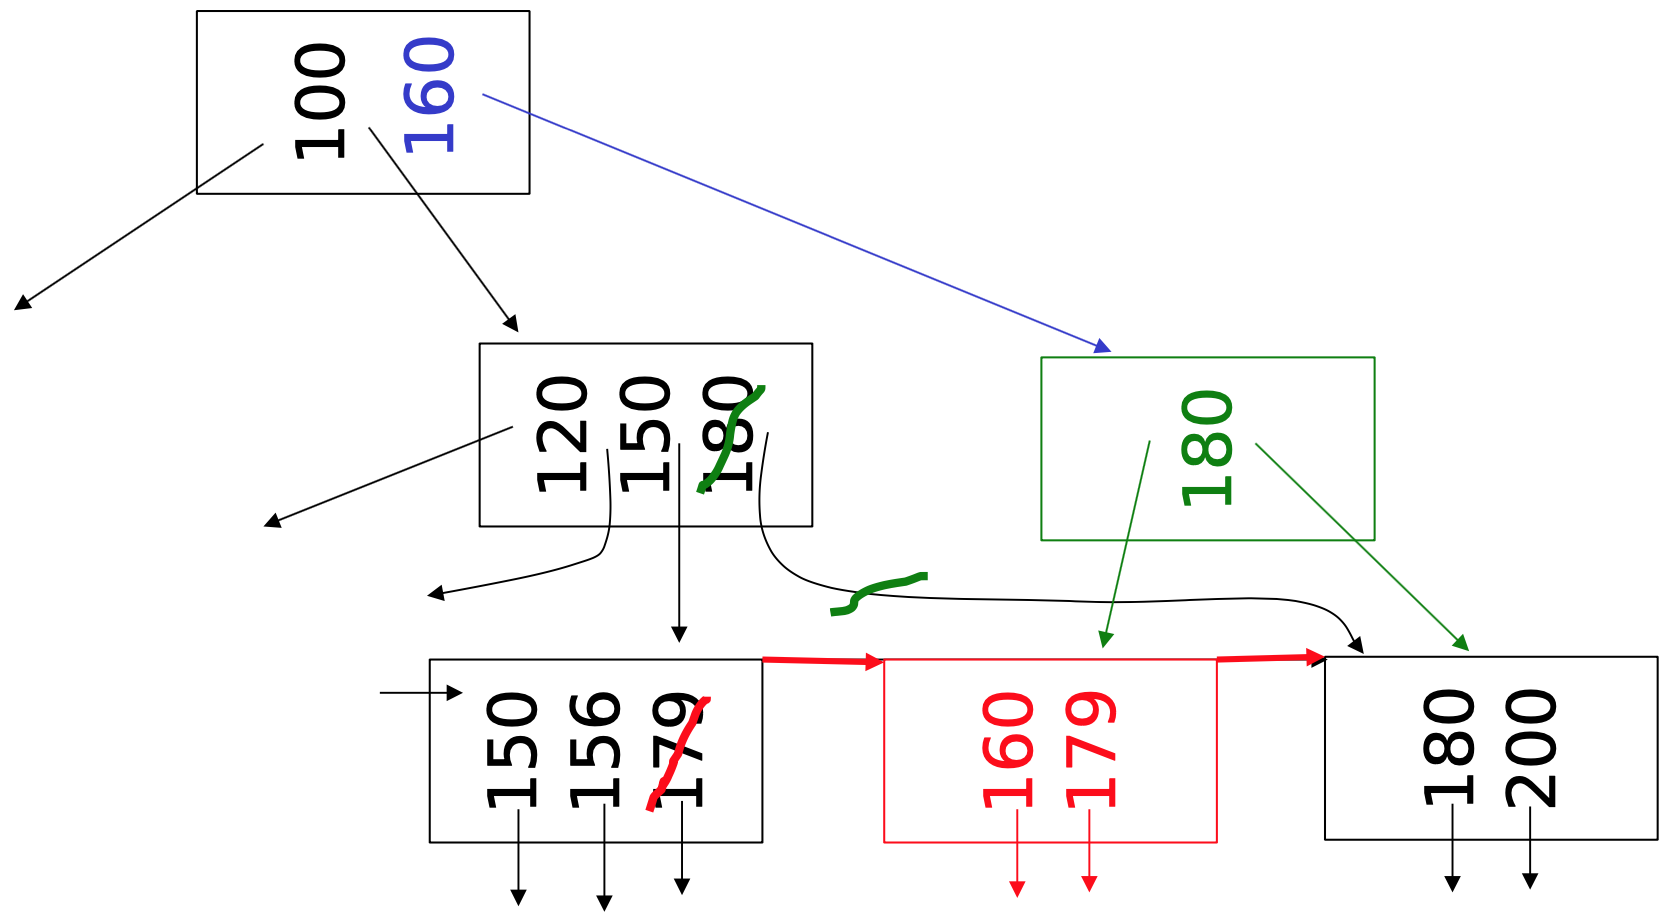
\includegraphics[scale=0.25]{img/img38.png}
\end{wrapfigure}
Now in scenario (c) the parents of the leaf where we want to insert doesn't have enough space to add a pointer like we did before. So after separating data into \textcolor{red}{2 half-full blocks}, when we need to add a pointers; we will create a \textcolor{ao}{new non-leaf block}. We separate the pointer in order to have at least 2 pointer by non-leaf. This new non-leaf must be designed by a pointer. We add these pointer into the grand-parents. The \textcolor{blue}{value} for the pointer is the smallest value that can be reached via the new pointer, meaning it's 160. The cost is the cost of searching + for each level we have to write into 2 blocks (in the worst case)\\


\begin{wrapfigure}[9]{l}{8.9cm}
\vspace{-5mm}
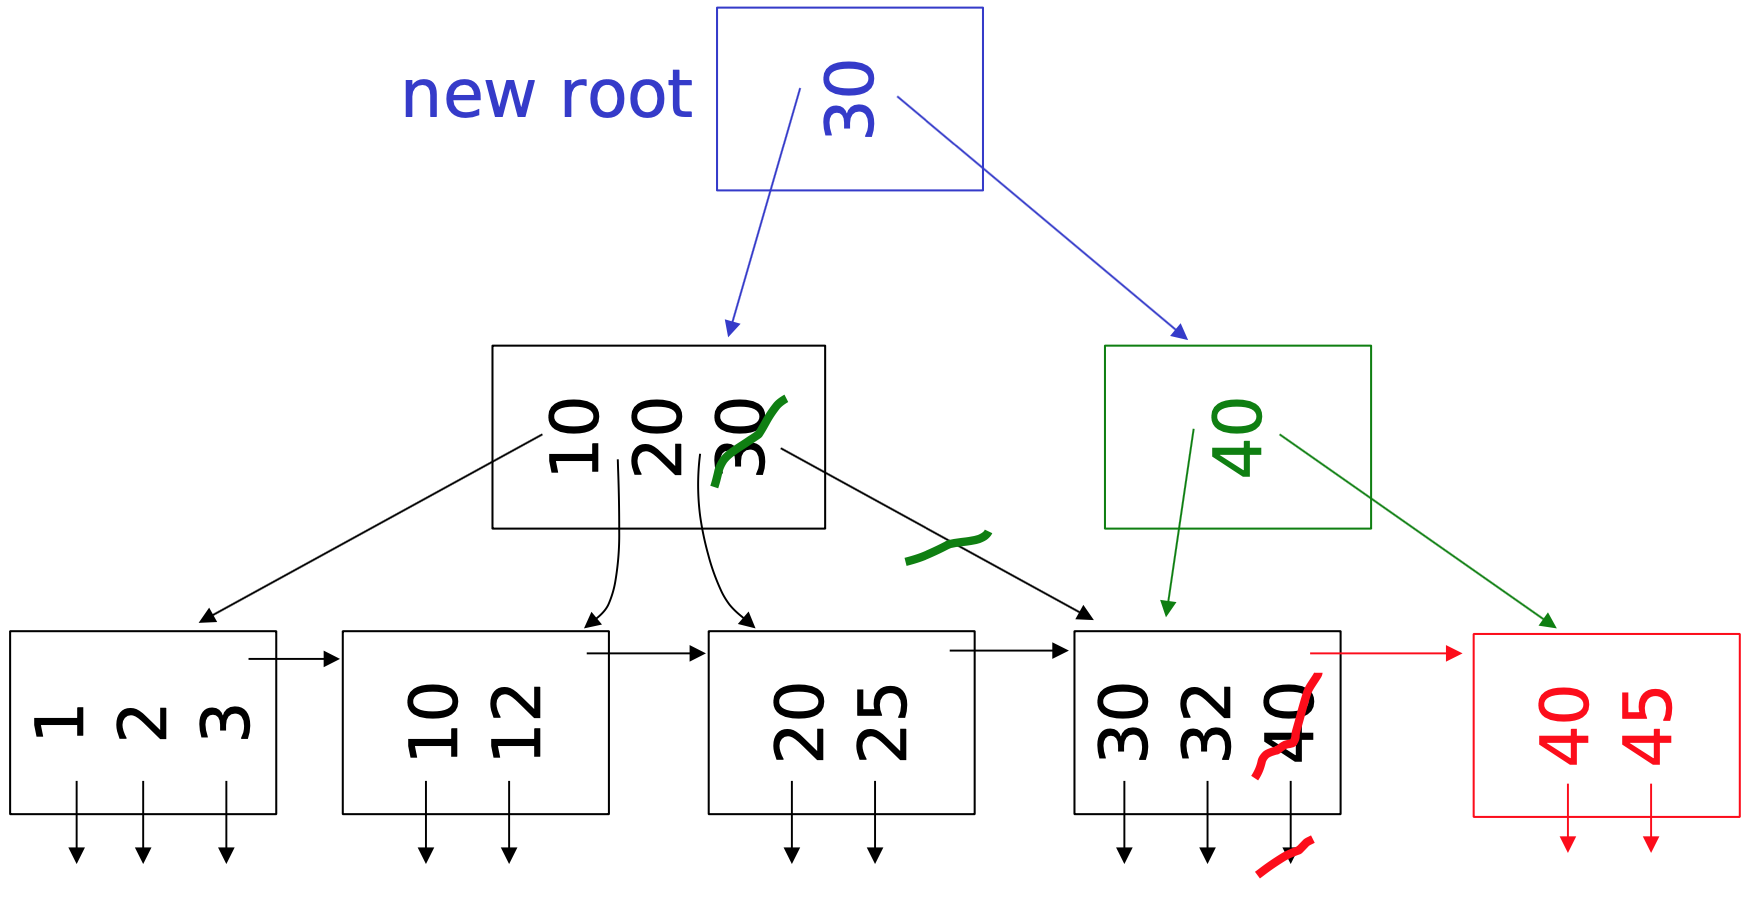
\includegraphics[scale=0.29]{img/img39.png}
\end{wrapfigure}
In scenario (d), the root is full and so we have to create a \textcolor{ao}{new block} at the same level, then a \textcolor{blue}{new root} as their parent, value in the root is the smallest value we can finc in the right branch. The cost is the cost of searching + wrtiting 2 blocks by level + writing one new root.\\
\\
\\
\paragraph{Delete}
Deletion is also separated into 4 scenario : the simplest case is when after deletion the leaf is still half-full (a), nothing must be done. We could have a case where the leaf is not half-full and the leaf must be coalesce with neighboor (b) or we have to re-distribute keys (c) or we have case (b) or (c) at non-leaf. Note : all the following examples are done with n = 4.\\

\begin{wrapfigure}[9]{r}{8.9cm}
\vspace{-5mm}
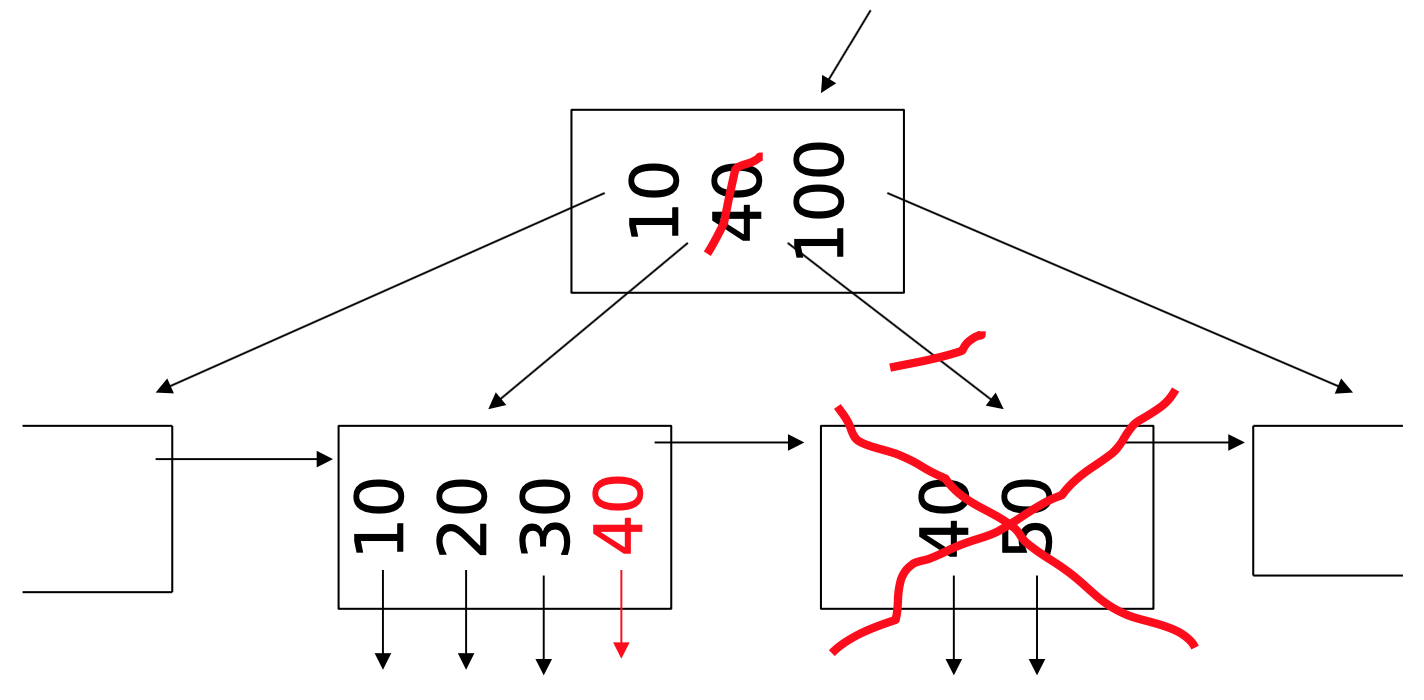
\includegraphics[scale=0.29]{img/img40.png}
\end{wrapfigure}
Here is an example for scenario (b) were we delete 50, after deletion there is only 1 pointers to data so the leaf can't stay that way. We look to siblings to see if remaining pointer can be added there. This means that the pointer for the deleted block must be deleted to.\\
\\

\begin{wrapfigure}[9]{r}{8.9cm}
\vspace{-5mm}
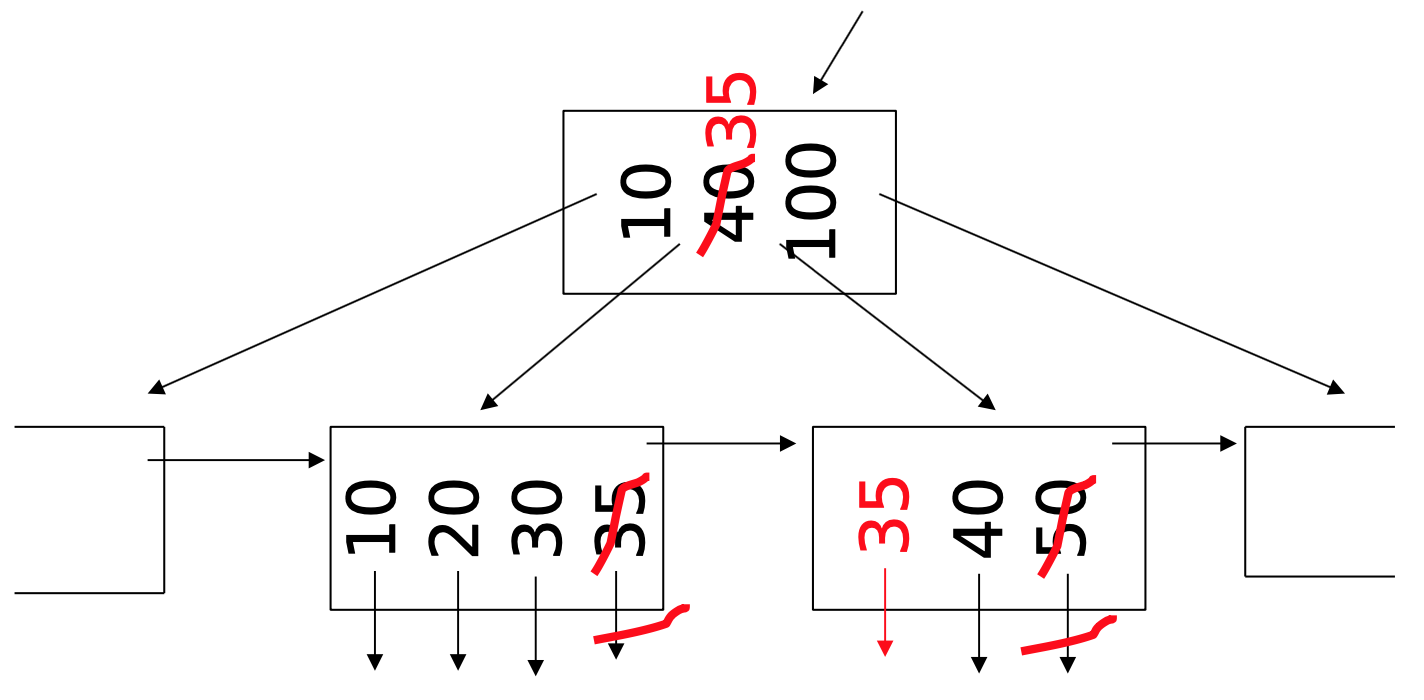
\includegraphics[scale=0.29]{img/img41.png}
\end{wrapfigure}
Scenario (c) occurs when the sibling are full or don't have available space for all the remaining pointers. This means the the number of pointers in the sibling + number of remaining pointers must be at least enough for 2 half-full leaf. So we redistribute the keys. The value in the \textcolor{red}{parent} must also be modified.\\
\\

\begin{wrapfigure}[9]{l}{7.7cm}
\vspace{-5mm}
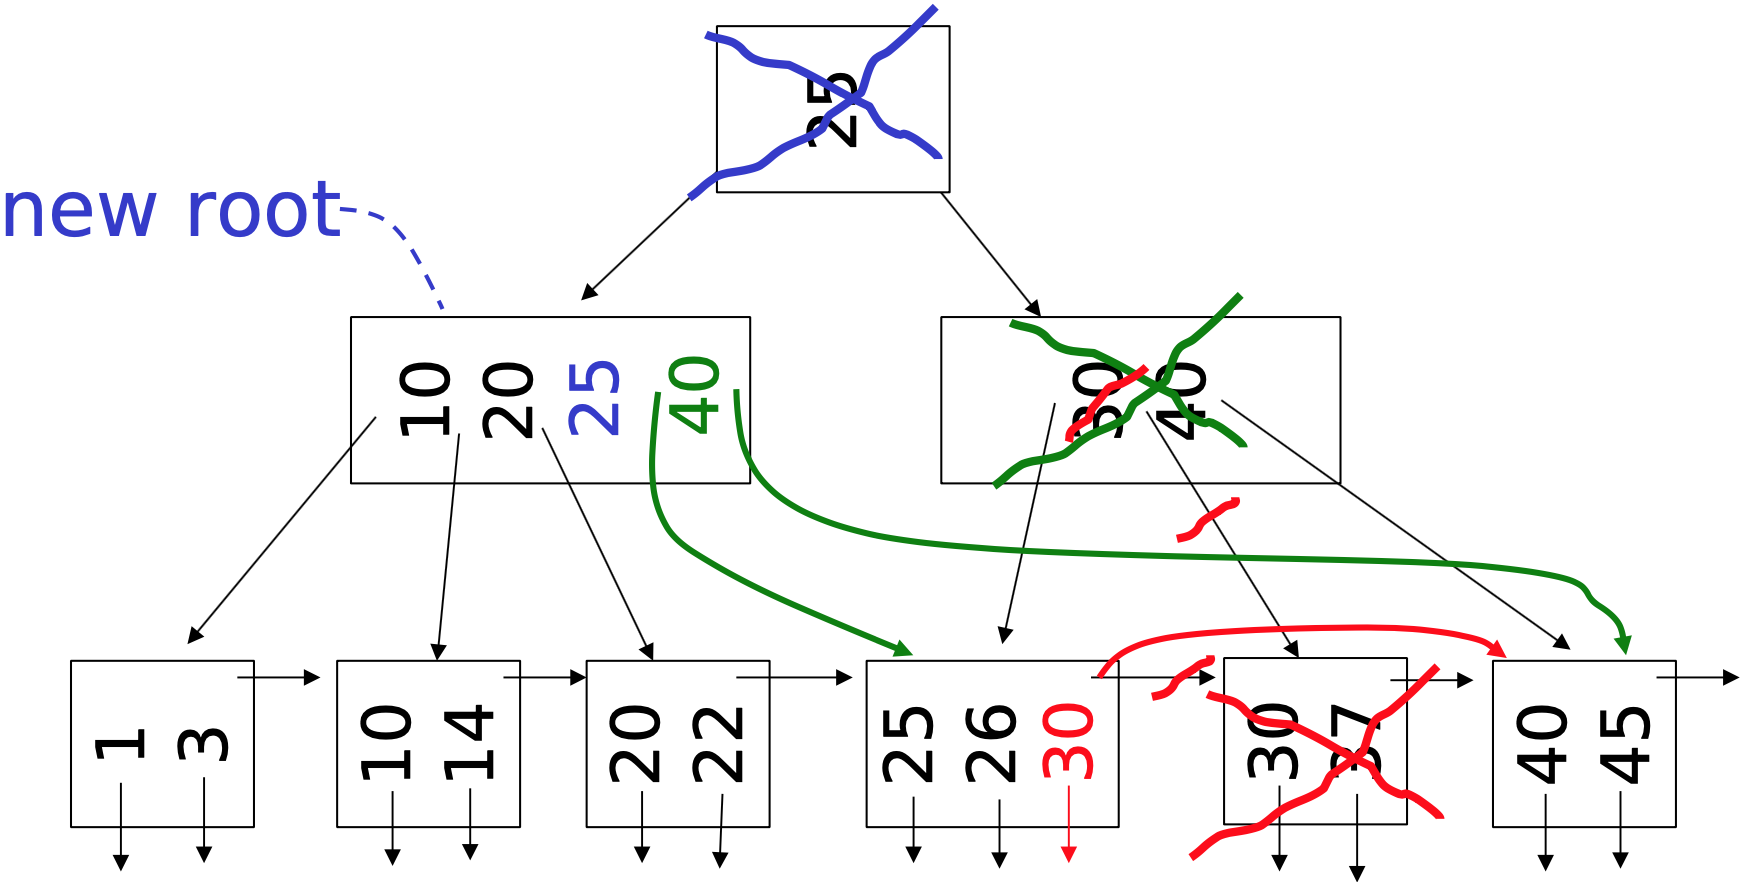
\includegraphics[scale=0.25]{img/img42.png}
\end{wrapfigure}
In scenario (d) we consider what happens when the previous situation occurs for non-leaf nodes. When we remove pointer for the $30-37$ block, the parent nodes don't have enough pointers anymore. We can then move the single remaining pointer to its \textcolor{ao}{sibling}. Then we need to remove the pointer toward $30-40$ from the \textcolor{blue}{root}. We must then modify the value in the ex-$10-20-40$ nodes so that it becomes the new root.\\


\subsection{Hashing - lecture 4}
This data structure doesn't work by sorting data (like index tree).
Concept of hashing is to process a key with an hashing function : key $\rightarrow$ h(key). The key is a number. Key are stocked in the bucket corresponding to their hashkey. Typicall size of bucket is 1 disk block. When we search for a record, we hash it then we know we only have to search in the bucket corresponding to that key and not in the whole database.\\
There is 2 ways to do things, either we stock the whole record in the bucket or just the search key and a pointer to where the record is. We use 2nd alternative for secondary search key because we assume data is already stored somewhere else and we just want another index, ne need to waste space.\\
There is a lot of already existing hash function, a good hash function gives us the same number of keys by bucket for every buckets no matter the data set, we don't want a situation where the whole database stored in the same bucket. Within a bucket we only keep the key sorted if CPU time is critical and insert/delete aren't too frequent.\\

\paragraph{Insertion}
We assume we can have 2 records by bucket max. We hash a few keys then find a new key that must be added to an already bucket. We could rebuild the hash table with more space but it's on secondary so it's really slow. The other solution is to add overflow blocks (like in index).

\paragraph{Deletion}
When we remove a element of a bucket with overflow blocks attached, element in the overflow block can be moved to try to reduce the number of overflow blocks.\\
We like to minimize the number of overflow blocks because if we have too much of them then it's like searching directly in the database, hashing become useless. We want to keep the length of the overflow block chains as small as possible. If the chains length become too big then we recreate a bigger hashtable\\

\begin{center}
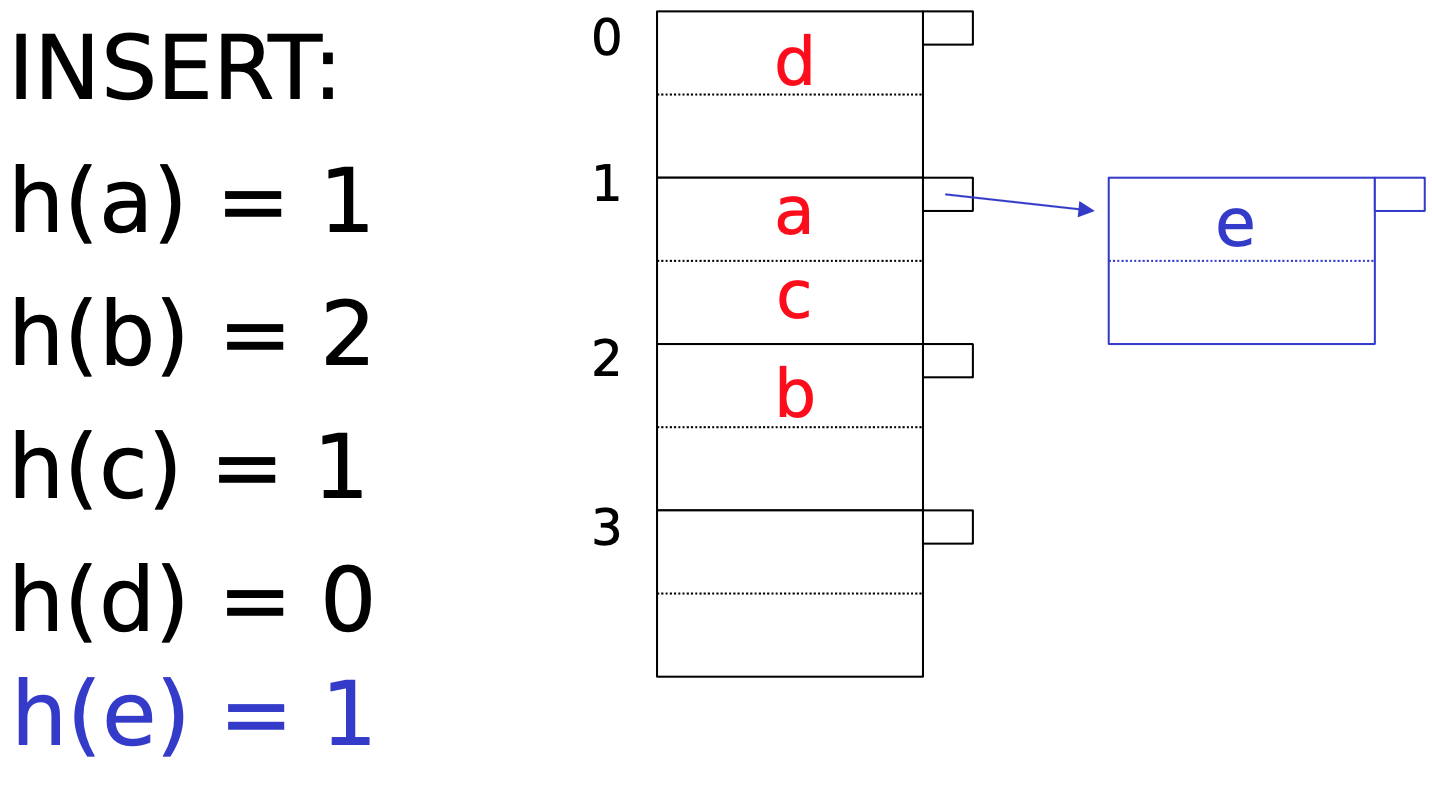
\includegraphics[scale=0.2]{img/img43.png}
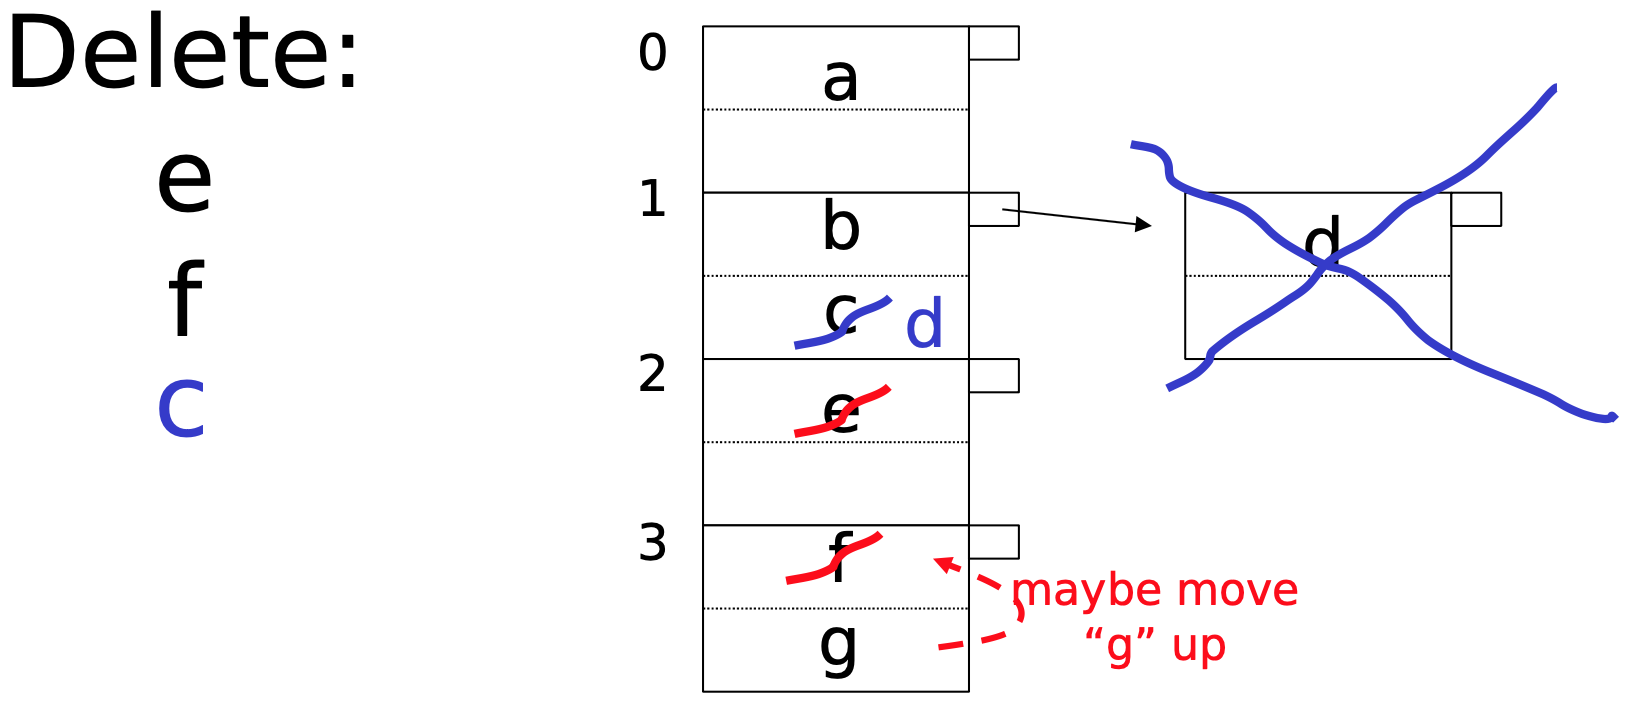
\includegraphics[scale=0.2]{img/img44.png}
\captionof{figure}{Example of insertion (left) and deletion (right)}
\end{center}

A good rule is that we try to keep space utilization between 50\% and 80$\%$. Where utilization is $\dfrac{\# \text{keys used}}{\text{total} \# \text{keys that fit}}$. Below 50$\%$ we're waisting space and over 80$\%$ the overflows become significant.

\subsubsection{Dynamic hashing}
Dynamic hashing is a way to cope gracefully with growth without having problem of overflow and reorganisation. There is essentially to way type of dynamic hashing : Extensible and Linear.

\paragraph{Extensible hashing}

\begin{wrapfigure}[7]{r}{6.5cm}
\vspace{-5mm}
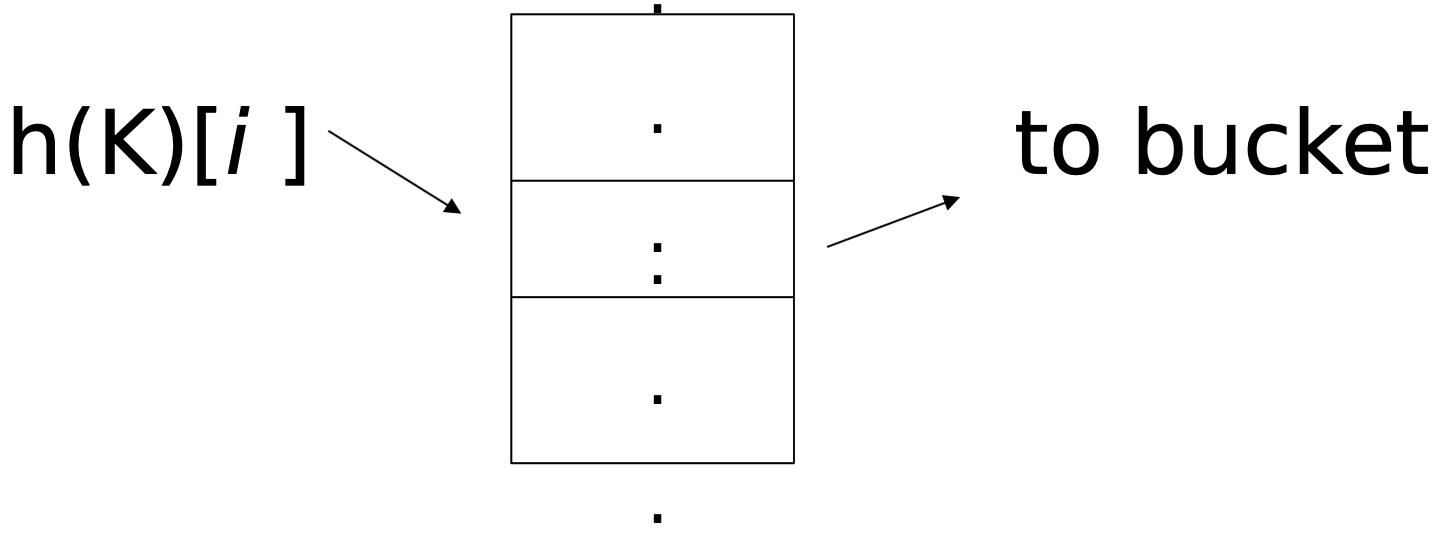
\includegraphics[scale=0.3]{img/img45.png}
\end{wrapfigure}
hash function gives a key with a certain number of bits. In extensible hashing we use only $i$ bits on the $b$ bits available but $i$ groxs over time. We only look at the $i$ most significant bits of the hash key. Also extensible hashing use an extra layer, a directory "between" the hashed key and the buckets. For an hashed key and a $i$ we look in the directory to know which bucket we should consult. The directory is an array of pointer.\\
\\
In the example below we see that first, we had $i=1$ and the corresponding directory with the address of buckets 0 and 1. But when we want to insert $1010$ there is not enough space. So $i$ increase to 2 and we create a \textcolor{blue}{new directory} with pointer toward bucket $00,01,10,11$. The element $1100$ move to the corresponding bucket and there is now space for $1010$.\\ 
Note : pointers for $00$ and $01$ are the same because this bucket still use $i=1$ since there was no need change (each bucket keep track of which $i$ it uses). If we want to add more records beginning with 0 then this bucket will split when necessary.
\begin{center}
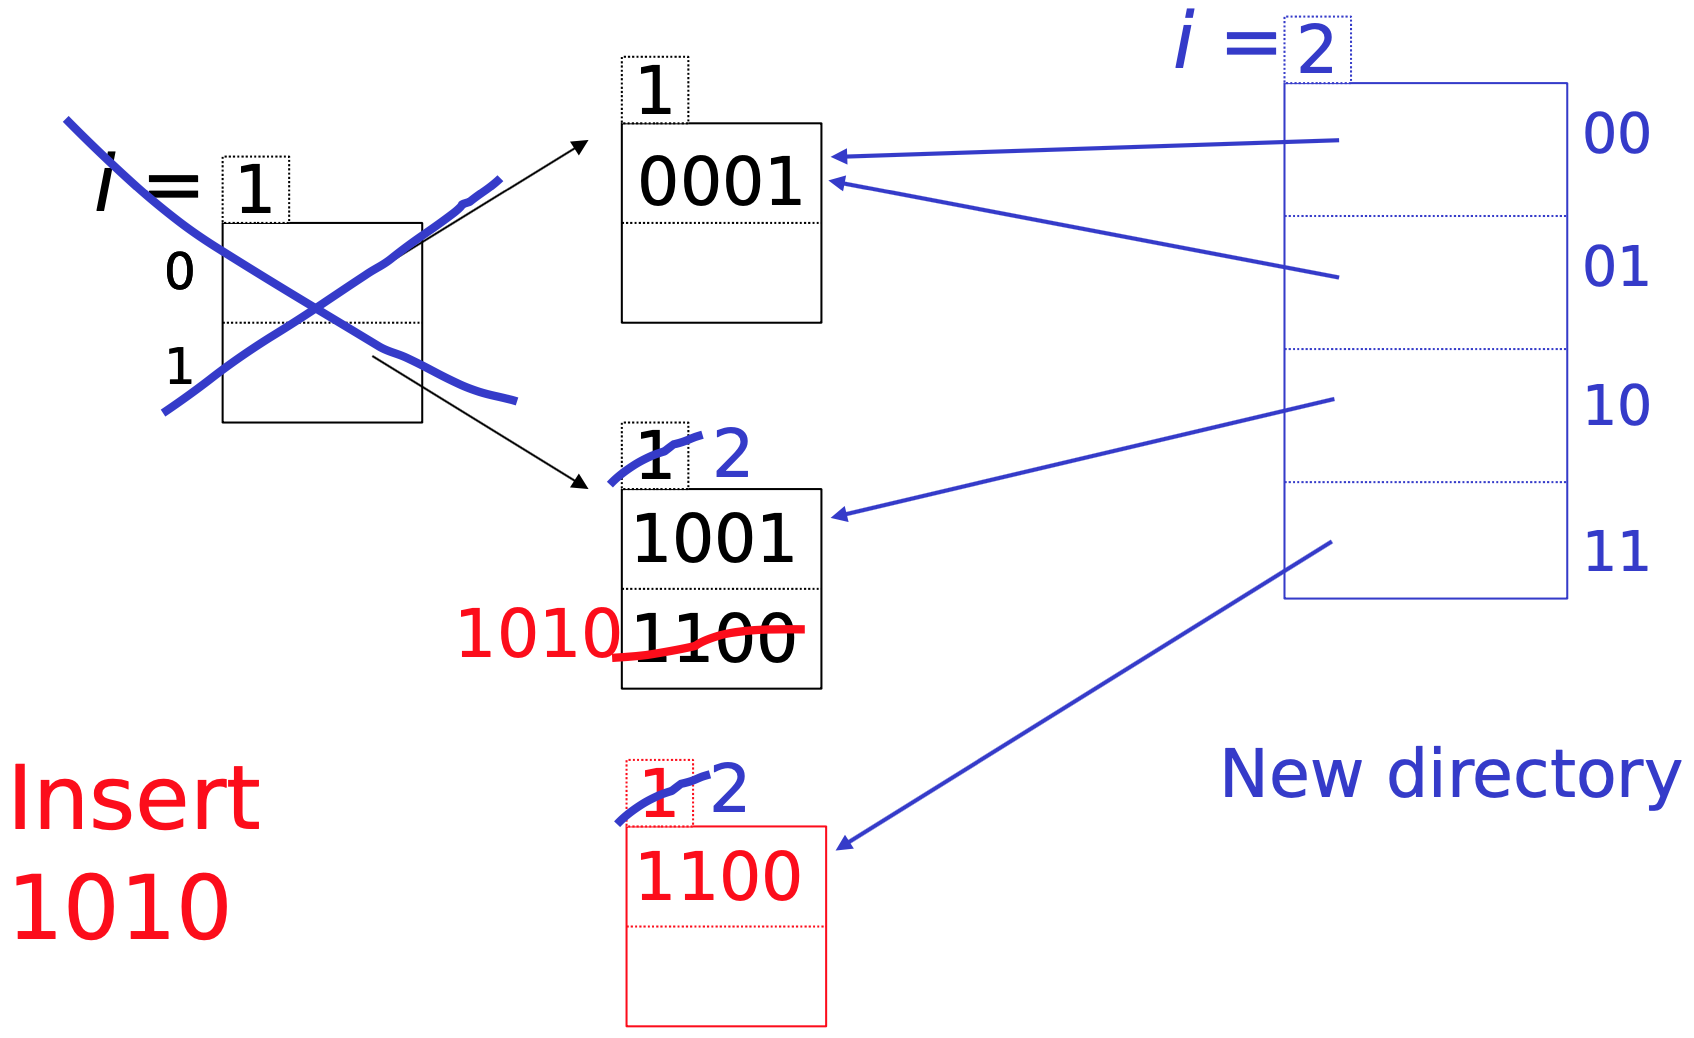
\includegraphics[scale=0.3]{img/img46.png}
\end{center}
If we wanted to add one more record beginning with $100$ then there wouldn't be enough space in the $10$ bucket and we should go to $i=3$, create a new directory, redistribute the records ...\\
\\

When deleting records there are 2 approach possible : first we assume that another record will be inserted shortly after and don't try to merge blocks. Or we can try to merge blocks and cut the directory is possible. It is just reversing the insertion procedure.\\

Exentisble hasing is good for handling growing files with less wasted space and no need for full reorganization, we just modify a few blocks at a time. However it involves indirection which not a problem if the directory fits in memoru but the directory doubles in size when it grows. If the directory doesn't fit in memory then this hashing is gonna be a bit useless, we have a lot more I/O.

\paragraph{Linear hashing}
Like in Extensible hashing we only look at $i$ of the bits but here we look at the $i$ \emph{least} significant bits. Here we don't use a directory but the number of buckets used will grow linearly. If $n$ is the id of the largest buckets in use (starting at 0) then we have the constraint : $2^{i-1} \leq n+1 \leq 2^i$\\

\paragraph{Insertion}
The rule to search for/insert a new element is as follow : \\
$$\text{If } h(k)[i] \leq n \text{, then look at bucket } h(k)[i]$$
$$\text{ else, look at bucket } h(k)[i] - 2^{i-1}$$
The last part simply means that we flipp the most significant bit of the $i$ suffixe. If we want to add record to a full bucket then we use overflow blocks (they are allowed here).
\begin{center}
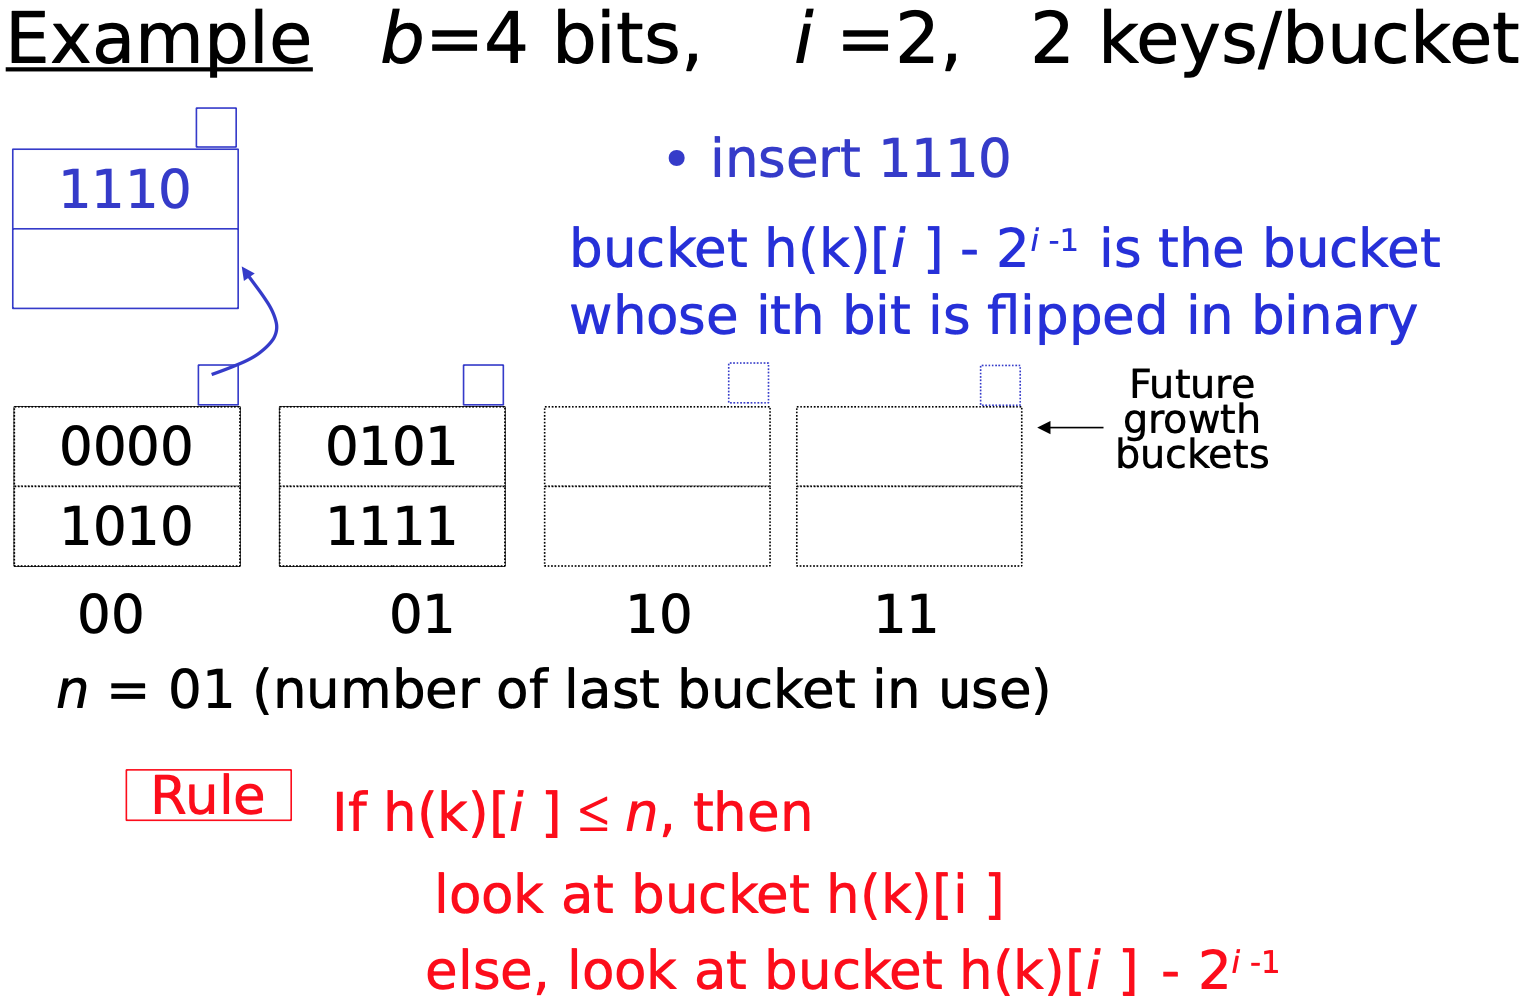
\includegraphics[scale=0.25]{img/img47.png}
\end{center}

When the number of overflow becomes too big, we're gonna grow the index but we don't need a full reorganisation. If we increase $n$ from $01$ to $10$ the data that should have been in $10$ when added is only in the bucket $00$ since we used the rule. It means we only have to scan through 1 bucket to reorganise the database correctly. And the length of the overflow in bucket $00$ decrease. The rule still applies once we're done with the reorganisation.\\
If we increase $n$ once again to $11$ then we just have to sort the key in bucket $01$. After that if we want to increase $n$ again, then $i$ will have to increase as well.\\

When we had $i = 2$ we never looked at the third bit, meaning in bucket $00$ we can have $100$ or $000$. When $n$ goes to $100$ we just have to reorganise the $00$ bucket and moves the key with $100$, all the others bucket are already organised !
\begin{center}
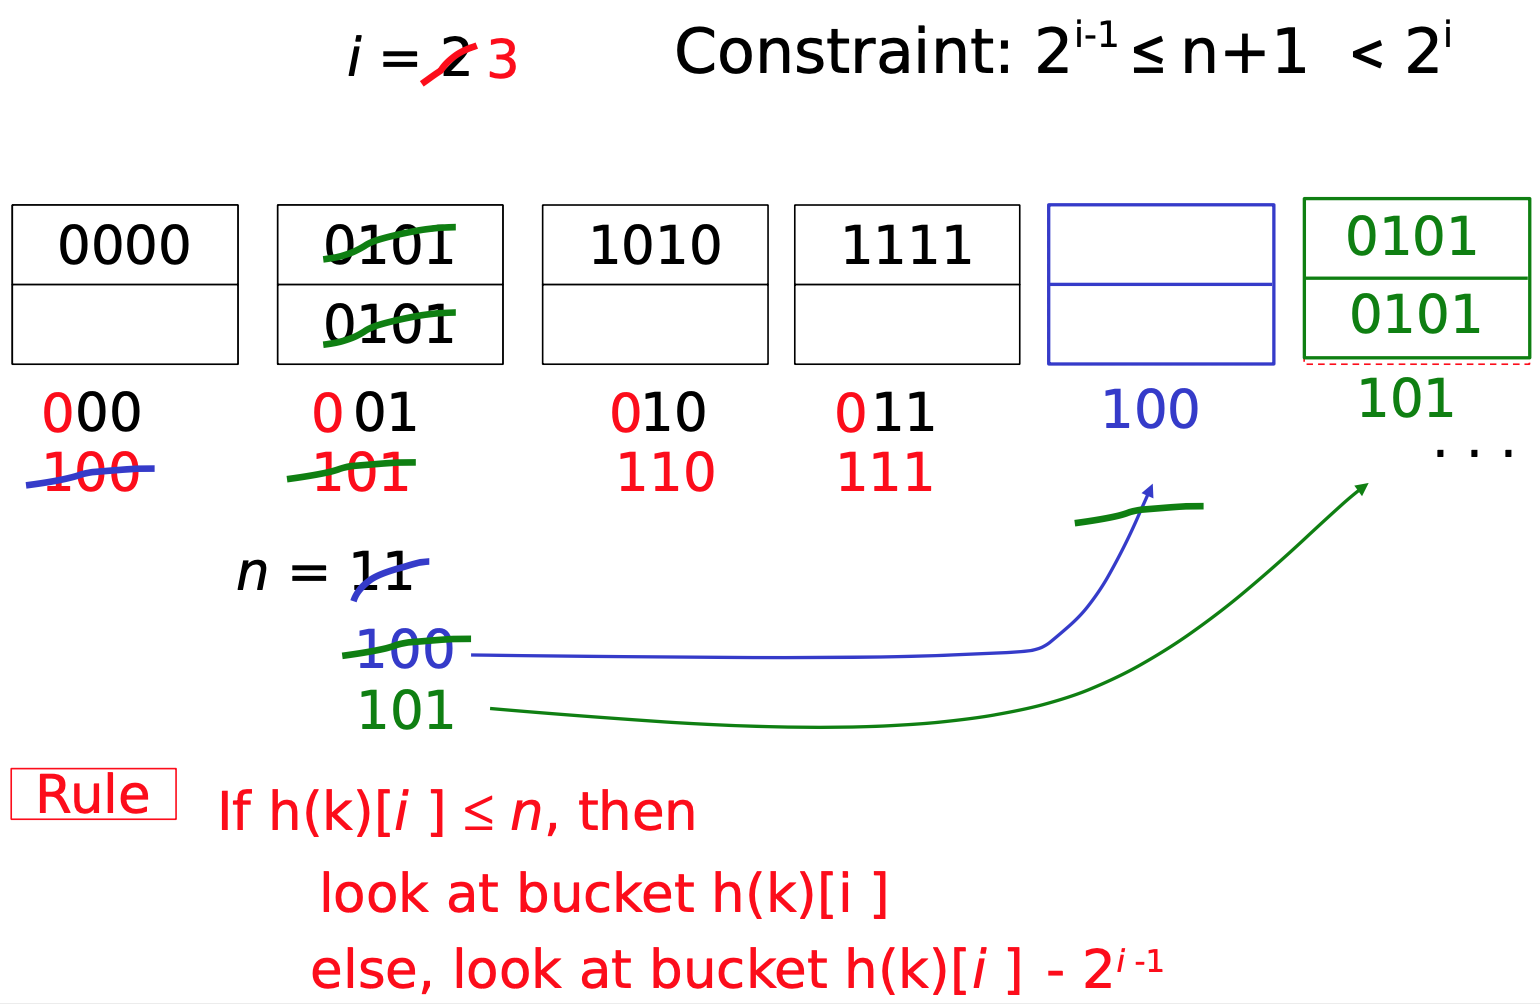
\includegraphics[scale=0.25]{img/img48.png}
\end{center}


To know when to expand the file we keep track of $U = \dfrac{\# records}{\# buckets}$, if $U >$ threshold then we increas $n$ (and $i$ if needed).\\
Linear hashing can handle growing file with less wasted space, no full reorganization and no indirection. However it still has overflow chains. 
Those overflow chain could mean we have a very full buffer with a long overflow chain but to resolve the situation we must increase $n$ a lot. That would be a waste of space.

\paragraph{BTree vss Hashing}
Hashing is good for selecting on a given key (extensive hashing is perfectly fine as long as the directory can be kept in memory) and BTree are good for ranged search (by default most system create a BTree when asked for an index).

\subsection{Multi-dimensional Index Structure - lecture 5}
\paragraph{Motivation}
Before we assumed that the search key was a single attribut but not always the case. We might need to do query in data warehouse which are repository of all data collected over time. Data warehouse are decision support system and are a bit different from traditional relational database. They usually integrate different database and access a lot of information. We want data available immediatly and for that we use cross-tabulation and data cubes that are their extension to multiple dimension. 
\begin{center}
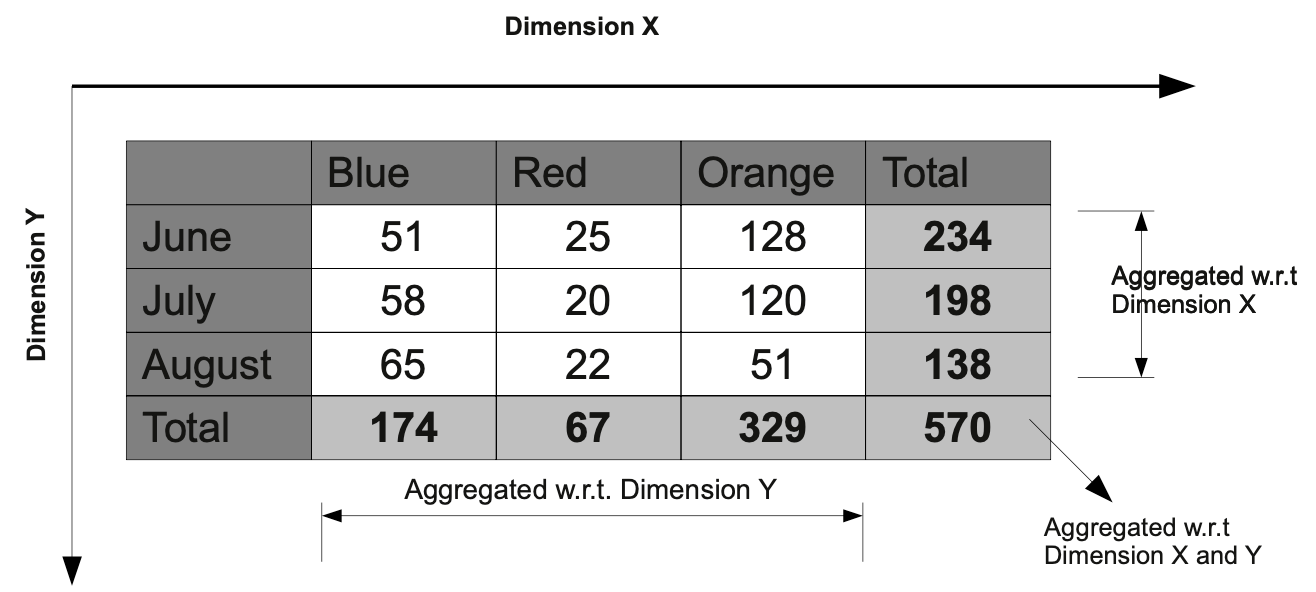
\includegraphics[scale=0.35]{img/img49.png}
\includegraphics[scale=0.35]{img/img50.png}
\captionof{figure}{cross-tab (left) and datacube (right)}
\end{center}
We might want to do some agregation operation on that datacube, for exemple group our data by semester, it's called the \textbf{roll-up} operation. The inverse is \textbf{drill-down} and for example would be to separate $Q$ into month of weeks.\\
Another things we can do is a \textbf{slice and dice} which is select only a part of the cube, for exemple only the data for Ireland and VCR :
\begin{center}
\includegraphics[scale=0.4]{img/img51.png}
\end{center}
Now how to implement this ? We could simply use a mutlidimensional array and to access a cell use notation cell[product, date, country]. It semms easy however the problem is that usually data isn't "dense" meaning our array would take a lot of space ($c^n$ if we have $n$ dimensions with $c$ possible values) but the major part of this space is empty. Taking that must space for few data is not a good idea. So we use alternative representation strategies that use sparse main memory index structures like search trees or hash table. And these can be speciallized to also work in secondary memory.\\
Data cube can be encoded as relational database where we can do the same operation (slicing, roll-up), however the SQL query can easily become very complex and not-readable.
These query will need to do search on multiple attribute so we need index structure that allow multiple keys $\longrightarrow$ \textbf{mutlidimensional indexes}.\\
\\
\paragraph{Multidimensional Indexes } are obviously used with data cube but also for spatial databse. Typical queries are : 
\begin{itemize}
\item point queries : we want the data at a precise point
\item : partial mathc : data that correspond to some criteria (=)
\item : dicing/range queries : data that correspond to some criteria (<,>)
\item : nearest-neighbour : data "closest" to a point
\end{itemize}

Why can't we use BTree or Hash table ?\\
\begin{wrapfigure}[9]{l}{5cm}
\vspace{-10mm}
\includegraphics[scale=0.37]{img/img52.png}
\end{wrapfigure}
\underline{BTree} assumes that key search can be ordered, we could choose to use the lexical order for a multidimensional search key : $$(x,y,z) \leq (x',y',z') \Leftrightarrow x < x' \vee (x=x' \wedge y=y') \vee (x=x' \wedge y=y' \wedge z\leq z')$$
On the left we can see how the values for an (age, salary) tuple will be parcoured. We can use the BTree to look for tuple where age $<$ 20 but we can't use it for tuple where sal $<$ 30, we will have to do a linear scan. We could produce 2 BTree but we would like to only need 1 for all queries.\\
\\
\underline{Hash table} assumes a hash function $h : keys \rightarrow \mathbb{N}$, for a multidimensional search key we could extend an hash function to tuple : 
$$h(x,y,z) = h(x) + h(y) + h(z)$$
In order to do a search for age $<$ 20, sal $<$ 30 or a search for age $< 20 \wedge$ sal $<$ 20; we would need a linear scan. Indeed the idea of a hash table is to spread the data so it's absolutly not usefull when we want to do range queries.\\
What we need for multidimensional indexes is a notion of \textbf{spatial proximity}. \\

So we need other index structure, the first one is called \textbf{Grid file} and is actually based on hashing (it use bucket). We consider that our data is a 2x2 matrix with points at some positions (so we have 2 keys). We will separate the points into bucket, the index structure itself only need to store th coordinate of the separation. So we need to know if we sear for index between 2 value on x and y, where do we need to search. Since the number of region is much smaller than the number of points we can stock the index in main memory. 
\begin{center}
\includegraphics[scale=0.45]{img/img53.png}
\end{center}
The line are drawn in a way that ensure we have more or less the same number 
of in each bucket. It means we need to scan the data in order to determine the optimal position position for the line. For insertion we just look in which bucket the point is supposed to go and add it, if the block is full aither we add overflow block or we create a new separator line. This is actually difficult to do because adding a new separator line also separate all the other aligned bucket. In general we just use overflow block. To delete a tuple we find the corresponding bucket and delete the tuple.\\
This method work well for point queries, partial match queries and range queries. We can potentially have a lot of bucket to check but we also have a lot of answer so it's okay. 
For nearest neighbourhood searching it works a little less well because we look in the bucket corresponding to the position but if that bucket is empty then we need to also look in the bucket around it untill we find neighbours. This method is still reasonable but the downside is that if the data is not well distibuted then we have lots of empty bucket (3 empty bucket in the example).\\

Another index structure is \textbf{partitioned Hash function}, we consider we have 1024 bucket available to build a hashing index for $(x,y,z)$. Each bucket's number  is represented using 10 bits and we determine the hash value as :
\begin{center}
\includegraphics[scale=0.4]{img/img54.png}
\end{center}
Point queries and partial queries work well. We determine the value of the bit where it's possible and look at all the bucket(s) that match. Even for partial queries it's more efficient than looking in all the buckets.
However there is no support for range queries or nearest-neighbour queries since hashing "disperses" the data. The advantage is that it takes less spaces than grid files.\\

\begin{wrapfigure}[9]{r}{7.5cm}
\vspace{-9mm}
\includegraphics[scale=0.4]{img/img55.png}
\end{wrapfigure}
\textbf{kd-Trees} work a bit like grid file except that we use line that don't go through all the space. We take a first line that part the data into 2 spaces with roughly the smae number of point. Then we divide each subspace in the same way. We do that iteratively untill each subspace ahs a number of points that fit in a block/bucket. Note : when we draw line we alternate the axis.\\
This grid can also be represented as a (binary) Tree, each node gives on wwhich axis we did the separation and for which value. This tree structure is actually the index.\\
When we want to insert (or delete) a point, we just have to follow the tree then add (remove) the point in the leaf, if there isn't enough space we add a new split. So this index method have good support for point queries but also reasonably good support for partial match queries and range queries, we can compare the range with the criteria in a nodes then on the next level we search in both subtree. We alternate on which level we can take a decision and which level we must look in both subtree. Nearest neighbours is has reasonable support, we look in the corresponding bucket then look into sibling if the bucket is empty, then uncles if the sibling are empty, ...\\
To stock this tree in secondary memory we usually limit ourselves to 2 children per node (to not have problem of balance) but we store multiple nodes in a single blocks.\\
The worst scenario in a kd-Tree is when the tree is completly unbalanced because the complexity of searching is proportionnel to the height of the tree.

The last index structure resolves this problem, it's called \textbf{R-Trees}. They're a proper generalization of BTree to multiple dimensions and are designed to index regions where a single point is also viewed as a region. We use bounding region to design a part of the map.
\begin{center}
\includegraphics[scale=0.5]{img/img56.png}
\end{center} 
When there isn't enough space in a block to insert a new element, we split the block in 2 and create a tree structure. The 2 new blocks created can overlap. If we search for an element in the overlapping part then we need to check in the two blocks. Here it's easier to keep the tree balanced because we can split and merge blocks when needed so our search time is always logarithmic.\\
This method has ideal support for "where-am-i" query, finding intersecting regions; good support for partial match and range queries and reasonable support for point queries and nearedt neighbours.
The main advantage is that it's balanced and very often used in practice if the data doesn't fit in memory. If the data fit in the main memory, kd-Tree are usually used.

\section{Physical Operators - lecture 6}

Here, we are at the "Physical query plan" part. We will assign to each logical operator (union, join, ...) a physical implementation algorithm. Those algorithms are called \textbf{physical operators}. For a single logical operator, there are multiple differents physical operator, each has a different cost. No implementation is always better than the others $\rightarrow$ comparaison on case-by-case basis.

\begin{center}
	\includegraphics[scale=0.35]{img/img1.png}
	\captionof{figure}{Query Compiler}
\end{center}

Data is storred on disk, divided into $D$ \textbf{blocks} of bytes. CPU can only work on data items that are in memory, memory can hold at most $M$ blocks of data ($M <<< D$).$\rightarrow$ Data must be transferred from disk to memory (transfer done in whole block), that's the most costly part. Cost of an algo is estimated by how many I/O must be donne on the disk.\\
Parameters used for the relation $R$, (note : 3 firsts are statistics that a DBMS regularly collect and stores in its system catalog):
\begin{itemize}
\item $B(R)$ : number of blocks that $R$ occupies on disk.
\item $T(R)$ : number of tuple in relation $R$
\item $V(R,A_1,...,A_n)$ : number of tuple in $R$ that have \textit{distinct value} for $A_1,...,A_n \rightarrow$ number of differents tuple after projecting $R$ on $A_1,...,A_n$
\item $M$ : the number of main memory buffer memory available
\end{itemize}

\subsection{Bag Union $R \cup_B S$}
reminder : bag means that we don't care if we have twice the same tuple in our database.\\

\begin{wrapfigure}[6]{l}{6.5cm}
\vspace{-5mm}
\includegraphics[scale=0.4]{img/img57.png}
\end{wrapfigure}
Here we have 2 relations $R$ and $S$ stocked on disk, there is 1 integer stocked into one memory block. In the main memory we reser 1 buffer frame $N$ to do the operation. We define the output as printing the tuple, so it's not counted as an I/O ( we never count the output-cost).\\
To do the union, we load the first block of $R$ into $N$ then output all its element, then do the same thing for the second block,... untill we outputed all of $R$ then we load the first block of $S$ and output all its element,... until we outputed all of $S$. For the exemple above, the print at the end are : 1,2,3,4,6,13,9,6,4,8,2,12.\\
\\
This operation only requiert one block of memoy available and for the I/O cost, since we have to load every block of $R$ and $S$ into memory we have a linear cost. Formally, we have :
\begin{itemize}
\item Cost : $B(R) + B(S)$ I/O operations
\item requiert that $M \geq 1$
\end{itemize}

\subsection{One-pass set union $R \cup_S S$}
reminder : set means we don't want to have duplicate. Here we're going to assume that the input relation don't have duplicate but we can have the same element in the 2 relations.\\

\begin{wrapfigure}[6]{r}{6.5cm}
\vspace{-5mm}
\includegraphics[scale=0.4]{img/img58.png}
\end{wrapfigure}
Here we assume we have $B(R) + 1$ free buffer frames in the main memory. We load all of $R$'s blocks into the memory and output their element. Then we load the first block of $S$ and output all its elements that do not occur in the frames containing $R$. After we repeat the process for all blocks of $S$. The output is 1,2,3,4,6,13,9,8,12.\\ 
\\
We can only use this algorithm when we have enough free space in memory, at least the size of the smallest relation + 1. Once again we have to load every block of the two relation. So we have :
\begin{itemize}
\item Cost : $B(R) + B(S)$ I/O
\item Requires $B(R) \prec M - 1$ (we assume $R$ is the smallest relation)
\end{itemize}
Rmq : we don't take into account the cost for checking if the elements of $S$ already appear in $R$. 

\subsection{Sort-based set union}
We can also compute the set union $R \cup_S S$ by sorting $R$ then sorting $S$ then iterating synchronously over $R$ and $S$ at each point loading 1 blocks of each relation in memory and inspecting 1 tuple of $R$ and $S$. Assuming we're currently looking at tuple $t_R$ in $R$ and $t_S$ in $S$, if $t_R < t_S$ then we output $t_R$ and move $t_R$ to the next tuple (loading a new block if needed), if $t_R > t_S$ then we output $t_S$ and move to the next tuple in $S$. If $t_R = t_S$ then we output $t_R$ and move $t_R$ and $t_S$ to the next tuple in $R$ and $S$.\\ 
The cost is still linear ($B(R) + B(S)$) and it requiers $M \geq 2$. 
We do this when we don't have enough space in memory, also we assume we have a good algorithm for sorting the relation when they are in main memory. This method is also called \textbf{merging}.\\

Usually the sorting is done by a \textbf{Multiway Merge-Sort}, this algorithm allow us to do a sort even when $R$ and $S$ dont fit in the memory.\\
\begin{enumerate}
\item In the first pass we read $M$ blocks at the same time from the input relation, sort these by means of a main-memory sorting algorithm, and write the sorted resulting sublist to disk. After the first pass we hence have $\frac{B(R)}{M}$ sorted sublists of $M$ blocks each.
\item In the 2nd pass, we merge the first $M$ sublists from the first pass into a single sublist of $M_2$ blocks. We do so by iterating synchronously over these $M$ sublists, keeping 1 block of each list into memory during this iteration. $\longrightarrow$ like when we compared tuple in $R$ and $S$ except that here we shouldn't have to tuple the same. \\
We then merge the next $M$ sublists into a single sublist, and continue until we have treated each sublist resulting from the first pass. After the second pass we hence have $\frac{B(R)}{M_2}$ sorted sublists of $M_2$ blocks each.
\item In the 3rd pass, we merge the first $M$ sublists from the 2nd pass (each of $M^2$ blocks) into a single sublist of $M_3$ blocks. We do so by iterating synchronously over these $M$ sublists, keeping 1 block of each list into memory during this iteration. We then merge the next $M$ sublists into a single sublist, and continue until we have treated each sublist resulting from the 2nd pass. After the 3rd pass, we have $\frac{B(R)}{m_3}$ sorted sublists of $M_3$ blocks each.
\item We keep doing new passes until we reach a single sorted list.
\end{enumerate}
For the cost now : at each pass we read and write the entire relation once, we stop doing passes when at the pass $x$ we have a single list of length $M^x = B(R)$ so $x = \lceil \log_M B(R) \rceil$. So the total cost is $2B(R) \lceil \log_M B(R) \rceil$.\\

This means that the total cost for the sort based union is the cost of sorting $R$, sorting $S$ then the cost of the union : 
$$2B(R) \lceil \log_M B(R) \rceil + 2B(S) \lceil \log_M B(S) \rceil + B(R) + B(S)$$
It requiers $M$ memory-buffers during the sorting and 2 memory-buffers for the synchronized iteration.\\
Note : in some case we could do the union when we finis the sort, for example if in the last step of the sort for $R$ we have 4 blocks and for $S$ we have 6 blocks with $M \geq 10$ then we could merge the 10 blocks at the same time.\\
The cost of this oprtimized version is slightly less for the sorting we have :\\
$2B(R) (\lceil \log_M B(R) \rceil - 1)$ and $2B(S) (\lceil \log_M B(S) \rceil - 1)$ since we have 1 pass less, the cost for the synchronized iteration doesn't change, so the new cost is :
$$2B(R) \lceil \log_M B(R) \rceil + 2B(S) \lceil \log_M B(S) \rceil - B(R) - B(S)$$
This optimization is only possible if the sum of $k$ (number of sublist of $R$ before the last pass) and $l$ (number of sublist of $S$ before the last pass) is inferior or equal at $M$. We have $k = \left\lceil \dfrac{B(R)}{M^{\lceil \log_M B(R) \rceil - 1}} \right\rceil$ and $l = \left\lceil \dfrac{B(S)}{M^{\lceil \log_M B(S) \rceil - 1}} \right\rceil$. So optimization is only possible when :
$$ \left\lceil \dfrac{B(R)}{M^{\lceil \log_M B(R) \rceil - 1}} \right\rceil + \left\lceil \dfrac{B(S)}{M^{\lceil \log_M B(S) \rceil - 1}} \right\rceil \leq M $$

\subsection{Hash-based set union}
Another way of compution the set union is to use a hash function on both relation then to compute the union bucket by bucket. However, the result of this union is not sorted.\\
The steps are : \\
Partition, using a hash function, $R$ in buckets of at most $M-1$ blocks each with $k$ the resulting number of buckets and $R_i$ the relation formed by the records in bucket $i$.\\
Then partttion, using the same hash function as before, $S$ in $k$ buckets with $S_i$ the relation formed by the records in bucket $i$.\\
Note that since we use the same hash function, if a tuple appears in $R$ and $S$ then it will appear in $R_i$ and $S_i$ with the same $i$.\\
Now we can compute the set union by calculating set union of $R_i$ and $S_i$ for every $i \in 1,...,k$. Since every $R_i$ contains at most $M - 1$ blocks, we can use the one-pass algorithm.\\
\\

How do we partition $R$ into buckets of at most $M-1$ blocks ?\\
First we use $M$ buffers to has $R$ into $M-1$ buckets. One buffer is used to load $R$ block by block, the $M-1$ other buffer are used to fill the block with the elements that hash into the $M-1$ buckets. Each time a blocks of one of the bucket is full, we write it in the disk. We procede like this until we have $R$ hashed into $M-1$ buckets.\\ 
Then we can repeat the process on each of the $M-1$ buckets, using a different hash function (if we don't we're gonna have exactly the same result). We repeat the process untill all the buckets we obtained have at most $M-1$ blocks.\\

If we assume that the hash function(s) distribute the records uniformly, we have $M-1$ bucket of $\dfrac{B(R)}{M-1}$ blocks after 1 pass, $(M-1)^2$ buckets of $\dfrac{B(R)}{(M-1)^2}$ blocks after the second pass, ... . Which means if we have buckets of $M-1$ blocks after $k$ passes then we have :
$$\begin{array}{rl}
\dfrac{B(R)}{(M-1)^k} & \leq M-1 \\
B(R) & \leq (M-1)^{1+k} \\
\log_{M-1} (B(R)) & \leq 1 + k \\
\end{array}$$
So the minimal value possible for $k$ is $\lceil \log_{M-1} B(R) - 1 \rceil$ and in every pass we read and writ $R$ once. So the total cost is :
$$2B(R) \lceil \log_{M-1} B(R) - 1 \rceil$$

Which means we can now compute the total cost of hash-based set union : we have the cost for each partition which are $2B(R) \lceil \log_{M-1} B(R) - 1 \rceil$ and $2B(S) \lceil \log_{M-1} \textcolor{red}{B(R)} - 1 \rceil$ (rmq : we have log of $B(R)$ because we only need to partition $S$ in as many buckets as $R$), then the cost for the one-pass set union on each $R_i$ and $S_i$ is $B(R) + B(S)$. The total is 
$$2B(R) \lceil \log_{M-1} B(R) - 1 \rceil + 2B(S) \lceil \log_{M-1} B(R) - 1 \rceil + B(R) + B(S)$$
note : in the book there is a particular case when we only need one pass for the hashing (only ok if $\dfrac{B(R)}{M-1} \leq M-1$ or approximatly $B(R) \leq M^2$), in that case the cost formula becomes $3B(R) + 3B(S)$.

\subsection{One-pass Join}
If we have $M-1 \geq B(R)$ then we can compute a join $R(X,Y) \Join S(Y,Z)$ by loading $R$ into the memory; then for each block $B_S$ in $S$, we load it in memory, for each tuple $t_S$ in the block we search for matching tuple $t_R$ in the memory blocks that contain $R$ and if we find a matching tuple, we output $t_R \Join t_S$.\\
The cost is $B(R) + B(S)$ since we need to read once $R$ and $S$. We don't take into account the cost for finding the matching tuple of each $t_S$.
It requiers $B(R) \leq M_1$.

\subsection{Nested Loop Join}
If we can't fit $R$ in memory (because $M-1 < B(R)$) then we can do a nested join. It's exactly the same process except that rather than putting $R$ in memory we just put the first $M-1$ blocks. Once the did the join with all the blocks of $S$ for this first segment of $R$ we put the $M-1$ next blocks of $R$ in memory and repeat the process.\\
The cost change obviously, we still need to read $R$ once the now we also need to read $S$ as many times as the number of segments of $M-1$ blocks in $R$. The cost becomes $B(R) + B(S) \times \dfrac{B(R)}{M-1}$, it's a quadratic cost which is very bad.

\subsection{Sort-merge Join}
It works essentialy like the sort-based set union : we sort $R$ \textcolor{red}{on attribute $Y$}, sort $S$ \textcolor{red}{on attribute $Y$} then iterate synchronously on $R$ and $S$, keeping 1 block of each relation in memory at all times, and at each point inspecting a single tuple from $R$ and $S$. 
Assume that we are currently at tuple $t_R$ in $R$ and at tuple $t_S$ in $S$ : 
\begin{itemize}
\item if $t_R.Y < t_S.Y$ then we advance the pointer $t_R$ to the next tuple in $R$ (possibly loading the next block of $R$ if necessary).
\item if $t_R.Y > t_S.Y$ then we advance the pointer $t_S$ to the next tuple in $S$ (possibly loading the next block of $S$ if necessary)).
\item if $t_R.Y = t_S.Y$ then we output $t_R \Join t'_S$ for each tuple $t'_S$ following $t_S$ (including $t_S$ itself) that satisfies $t'_S.Y = t_S.Y$. It is possible that we need to read the following blocks in $S$. Finally, we advance $t_R $to the next tuple in $R$, and rewind our pointer in $S$ to $t_S$.
\end{itemize}
The cost here is much better. It depends on the number of tuples with equal values for $Y$ . The worst case is when all tuples in $R$ and $S$ have the same $Y $-value. The cost is then $B(R) \Join B(S)$ plus the cost for sorting $R$ and $S$.\\
\\
If the join is perfomed on foreign key attribute (often the case) then there is only one tuple with this attribute and we don't need to reset the pointer in $S$ if we choose $R$ as the relation with the foreign key attribute. In that case the cost analysis is similar to the cost for a sort-based set union and the same optimization that remove $2B(R) + 2B(S)$ is possible.\\
\\
rmq : When $R$ (or $S$) has a BTree index on $Y$ then we don't have to sort $R$ ($S$) because the leaves of the BTree gives us $R$ ($S$) sorted on $Y$.

\subsection{Hash-Join}
It works essentially like the hash-based set union, the result is unsorted on the $Y$ attribute contrarly to the sort-merge join.\\
\\
First we partition, by hashing \textcolor{red}{the $Y$-attribute}, $R$ into buckets of at most $M - 1$ blocks each with $k$ the number of buckets required and $R_i$ the relation formed by the blocks in bucket $i$.\\
Then we partition, by hashing \textcolor{red}{the $Y$-attribute} using the same hash function as before $S$ into $k$ buckets. Where $S-i$ is the relation formed by the blocks in bucket $i$. Note : since we use the same hash function(s), the records in $R_i$ and $S_i$ have the same hash value. So a tuple $t_R \in R$ matches the $Y$ attribute of tuple $t_S \in S$ if, and only if, there is a bucket $i$ such taht $t_R \in R_i$ and $t_S \in S_i$.\\
\\
The last step is computing the join by calculating the join of $R_i$ and $S_i$ for every $i \in 1,...,k$. Since every $R_i$ has at most $M-1$ blocks, we can use the one-pass algorithm.\\

The cost is calculated exactly the same way as for the hash-based set union $\longrightarrow$  cost of the 2 hashing + cost of the join on the buckets.


\subsection{Index-Join}
In this case we assume that $S$ has an index on attribute $Y$. It means we can perfom the join by iterating on $R$ and for every tuple $t_R$, we search for the matching tuples $t_S$ in $S$ using the index. \\

The cost of this algo will depend on the cost of searching gor a tuple in the index•\\
If the index is a BTree then the cost for searching depends on the high of the BTree. If the index is a hash table then the cost depends on the number of overflow blocks. So we're gonna make a simplfying assumption and say that the cost of doing the search is going to be dominated by the cost of reading the matching tuples found.\\
There are 2 possibilities : if the index is clustered (BTree : at the leaves we have the data themselves) we estimate that for a tuple in $R$ the cost of reading all of the matching tuples in $S$ is $\lceil B(S) / V(S,Y) \rceil$, we need one I/O by blocks with the interesting tuples; however if the index is unclustered (BTree : at the leaves we have pointers to the data) then the cost for reading the intersting tuples in $S$ is $\lceil T(S) / V(S,Y) \rceil$, we need one I/O by tuples !\\
So the total cost is :
\begin{itemize}
\item index $Y$ is clustered : 
$$b(R) + T(R) \times \dfrac{B(S)}{V(S,Y)}$$
\item index $Y$ is not clustered : 
$$b(R) + T(R) \times \dfrac{T(S)}{V(S,Y)}$$
\end{itemize}
Where $T(R)$ is the number of tuples in $R$. This can potentialy be worse than nested loop join because it is quadratic with the number of tuples rather than the number of blocks. However it has th potential to be really intersting if $T(R)$ is small.

\section{Cost-Based Plan Selection - lecture 7}
Now that we have a logical query plan and know the cost of the different operators, we can obtain a \textbf{physical query plan} by assigning to each node a physical operator.
\begin{center}
\includegraphics[scale=0.5]{img/img19.png}
\end{center} 
We want to obtain the physical plan with the smallest cost so we will need to compare, for every node and applicable operator, it's cost. We still use the parameter $B(R),T(R),V(R,A_1,...,A_n)$ and begin by estimate the cost for the leaf then rise in the tree. For every internal node $n$ we will compute $B(n), T(n), V(n,A_1,...,A_k)$ where $T(n)$ and $V(n,A_1,...,A_k)$ depends on the logical query plan and $B(n)$ can be computed given $T(n)$, the size of the tuples output by $n$ and the size of the block. The main challenge will be to determinate $T(n)$.

\subsection{Result size of Projection}
\underline{Formula :} $T(\pi_L (R)) = T(R)$\\
We use bag-based projection so the number of tuple doesn't change. However the lenght of the tuple can change when we remove columns.

\subsection{Result size of Selection}
\underline{Formula :} $T(\sigma_P (R)) = T(R) \times sel_P (R)$ 
with the \emph{selectivity} $sel_P (R)$ the estimated fraction of tuples in $R$ that satisfies $P$, so it's the estimate probability that a tuple in $R$ satisfies $P$. The estimation of $sel$ depends on $P$.

\begin{description}
\item[$P \equiv A = c$] : $sel_{A=c} (R) = \dfrac{1}{V(R,A)}$, there are $V(R,A)$ distinct value of $A$ in $R$, if there uniformely ditributed then the probability that a tuple has the value $c$ is $1/V(R,A)$. If we have better statistic and an histogram of the database then a better estimate is possible.
\item[$P \equiv A<c$] : $sel_{A<c}(R) = \frac{1}{2}$ or $sel_{A<c}(R) = \frac{1}{3}$, in the absence of more detailed statistic we use an heuristic.With more detailed statistic a better estimate is possible. For example if we know the range of $A$-values then we know how many values satisfies the condition.
\item[$P \equiv A \neq c$] : $sel_{A \neq c}(R) = \dfrac{V(R,A) - 1}{V(R,A)}$, it's 1 $- sel_{A=c}(R)$.
\item[$P \equiv \texttt{NOT } P_1$] : $sel_{\texttt{NOT } P_1}(R) = 1 - sel_{P_1}(R)$
\item[$P \equiv P_1 \texttt{ AND } P_2$] : $sel_{P_1 \texttt{ AND } P_2}(R) = sel_{P_1}(R) \times sel_{P_2}(R)$, this implicitky assume that $P_1$ and $P_2$ are indenpendent. The order doesn't matter.
\item[$P \equiv P_1 \texttt{ OR } P_2$] : $sel_{P_1 \texttt{ OR } P_2}(R) = \min (sel_{P_1}(R) + sel_{P_2}(R),1)$, the summ implicitly assumes that $P_1$ and $P_2$ are indenpendent and select disjoint sets of tuples even if it's not always the case.
\end{description}

\subsection{Result size of Cartesian product}
\underline{Formula :} $T(R \times S) = T(R) \times T(S)$

\subsection{Result size of Natural join}
It's a bit more complicated we do a join on $Y$ for $R(X,Y)$ and $S(Y,Z)$, differents cases are possible : $R$ and $S$ can have no $Y$ in common and then $T(R \Join S) = 0$, $Y$ might be the key of $S$ and a foreign key of $R$, so each tuple $R$ join with exactly 1 tuple of $S$ and then $T(R \Join S) = T(R)$, or all tuples of $R$ and $S$ can have the same $Y$-value and then $T(R \Join S) \approx T(R) \times T(S)$. The last case is unlikely because people aren't usually interested in cartesian product.\\
\\
We can do 2 simplifying assumption : if $V(R,Y) \leq V(S,Y)$ then every $Y$-value of $R$ will have a joining tuple in $S$; $V(R \Join S,A) = V(R,A)$ when $A$ is in $R$ and $V(R \Join S,A) = V(S,A)$ otherwise. With these assumption we can estimate that
\begin{itemize}
\item if $V(R,Y) \leq V(S,Y)$ : $T(R \Join S) = T(R) \times \dfrac{1}{V(S,Y)} \times T(S)$
\item if $V(S,Y) \leq V(R,Y)$ : $T(R \Join S) = T(R) \times \dfrac{1}{V(R,Y)} \times T(S)$
\end{itemize}
\underline{Formula :} $T(R \Join S) = T(R) \times T(S) \times \dfrac{1}{\max(V(R,Y),V(S,Y))}$\\
For the case where we have $R(X,Y_1,Y_2)$ and $S(Y_1,Y_2,Z)$ woth the join on $Y_1$ and $Y_2$, the various possibilities of inequality give 4 differents case and we can deduce a general formula.\\
\underline{Formula :} $T(R \Join S)  = \dfrac{T(R) \times T(S)) }{\max(V(R,Y_1),V(S,Y_1))\max(V(R,Y_2),V(S,Y_2))}$

\subsection{Join Ordering}
Join operator are binary so we can only join to relation at a time. To reduce the cost we need to execute the join that gives the less blocks first. This means that to have an optimal physical plan we would need to enumerate and compare every possible join ordering. The number of possible join ordering rapidly becomes enormous as the number of relation climb up. We will then only consider the possibilities for \textcolor{blue}{left-deep} join ordering.
\begin{center}
\includegraphics[scale=0.5]{img/img59.png}
\end{center}
Even with that reduction of possibilities, for a high number of relation it would still take more time to compute the best plan than to execute it. We would like to avoid that so we will use a greedy algorithm :\\
We work bottom-up by first assigning physical operator on the leaves, then to the parents of the leaves, etc and at each point choose the operator with the least cost.\\
When we reach a join operator we start by joining the 2 relations for which the best physical join algo has the smallest cost. Then add the remaining relations to the join beginning by the one with the smallest cost.\\
In some case the plan returned by the greedy algorithm doesn't give us the best result but it's good enough!\\
The result of the greedy algorithm is an execution tree where every node is a physical operator.\\
Some operator can be pipelined, which means that their output is directly passe as input of the next operator rather than writing/reading it on disk. This process reduce the number of I/O, the memory requirements and the response time. Some operator, called \emph{blocking}, can't be pipelined.


\section{Coping with System Failure - lecture 8}
When we use database, we want our data to be correct at all time. TO ensure so we can put integrity/consistency constraints that data must satisfy (eg : upper-bound on the age or salary of a person, domain valid for an attribute, relation that must be true between attribute,...). However the constraint can't always totally correspond to reality and ensure a "full correctness".\\
A \textbf{consistent state} is a state where all constraints are satisfied and a \textbf{consistent database} is a DB in a consistent state.\\
A database can't always be consistent. When we have to change data inside it we can only do 1 operation at a time and thus there can be moment where the database isn't consistent. A \textbf{transaction} is a collection of actions that preserve consistency. When we stop runnig transaction the database should be left consistent.\\
The constraint can be violated if there is a transaction bug, DBMS bug, hardware failure or some dumb data sharing. Here we will only see how to prevent/fix violation due to failure. In the failure model we consider we can have \emph{desired} or \emph{undesired} events and the \emph{undesired} ones can be \emph{expected} or \emph{unexpected}. The undesired expected events can be system crash due to memory lost or cpu halts then resets. Everything else is unexpected and we don't safeguard against it.\\
\\
\begin{wrapfigure}[6]{r}{6.5cm}
\vspace{-8mm}
\includegraphics[scale=0.37]{img/img60.png}
\end{wrapfigure}
The approach is to add low level check and redundancy to increase probability that the model holds. The storage hierarchy is defined with the memory and the disk. Different operation are defined :
\begin{description}
\item[Input($x$)] block containing $x \rightarrow$ memory
\item[Output($x$)] block containg $x \rightarrow$ disk
\item[Read$(x,t)$] do input($x$) if necessary \\ $t \leftarrow$ value of $x$ in block
\item[Write$(x,t)$] do input($x$) if necessary \\ value of $x$ in block $\leftarrow t$
\end{description}

The key problem is usually an unfinished operation, in the next example we have the constraint $A = B$. If there is a failure and the second output isn't done then $B$ doesn't change on disk and the constraint isn't satisfied.
\begin{center}
\includegraphics[scale=0.2]{img/img61.png}
\end{center}
It means we need \textcolor{red}{atomitcity}, all the actions of a transaction are executed or none are.

\subsection{Undo logging}
A first solution is to use a log where we keep tract of the old value. When a transaction begins we write it, then the set of instruction done then the end of the transaction. It there is an interruption we can check the log and undo all transaction that didn't end. A complication can arise if we did a operation then there is a crash and the operation ahdn't be recorded in the log. Thus there is a serie of undo logging rules :
\begin{enumerate}
\item For every action generate undo log record (containing old value)
\item Before $x$ is modified on disk, log records pertaining to $x$ must be on disk (write ahead loggin : \textbf{WAL})
\item Before commit is flushed to log, all writes of transaction must be reflected on disk
\end{enumerate}
The rules for recovery are :
\begin{enumerate}
\item Let S =  set of transactions with $<Ti, start>$ in log, but no $<Ti, commit>$ or $<Ti,abort>$ record in log
\item For each $<Ti,X,v>$ in log, in \textcolor{red}{reverse order} (latest $\rightarrow$ earliest)do:\\
if $Ti \in$ S then {write$(X,v)$ ; output$(X)$}
\item For each $Ti \in$ S do:\\
write $<Ti,abort>$ to log
\end{enumerate}
If we don't undo in reverse order then we could have the wrong value when a value has been modified more than 1 time.\\
If there is a failure during the recovery, it's no problem we can redo the recovery as many time as needed without changing the result (idempotent).\\

If the log grow too much we might want to delete the older entries. We can decide to have checkpoints : periodically we don't accept new transaction, wait until all running transaction have finished and flushed their modif to disk, flush all log records to disk(log), write \textit{checkpoint} record on disk (log) then resume accepting transaction.\\
Then in case of failure we only need to undo transaction younger than the last checkpoint and can remove the older part from the log.\\
The problem is that those checkpoints effectively shut down the system while waiting for the commit of the current transaction.\\

Another, more complex, technique called \textbf{nonquiescent checkpoint} is used. It allows new transaction during the checkpoint.
\begin{enumerate}
\item Write a log record $<\texttt{START CKPT} (T1,..., TK)>$ and flush the log. $T1...Tk$ identify the active transactions (not yet committed and written their changes to disk)
\item Wait until all of $T1 ... Tk$ commit or abort, but do not prohibit other transactions form starting
\item When all of $T1 ... Tk$ have completed,
write $<\texttt{END CKPT}>$ to log on disk (log)
\end{enumerate}
In case of failure, we can undo everything younger than the last \textcolor{blue}{completed} start checkpoint. All the older logs can be removed.

\subsection{Redo logging}
It's another way to use the logging :
\begin{enumerate}
\item For every action, generate redo log record (containing new value)
\item Before $X$ is modified on disk (DB), all log records for transaction that modified $X$ (including commit) must be on disk
\item Flush log at commit
\item Write END record after DB updates flushed to disk
\end{enumerate}
And the recovery rules are :
\begin{enumerate}
\item Let S = set of transactions with $<Ti, commit>$ (and no $<Ti, end>$) in log
\item For each $<Ti,X,v>$ in log, in forward order (earliest $\rightarrow$ latest) do:\\
if $Ti \in$ S then {Write$(X,v)$ ; Output$(X)$}
\item For each $Ti \in$ S, write $<Ti, end>$
\end{enumerate}

Redo logging can also use non-quiescent checkpoint :
\begin{enumerate}
\item  Write a log record $<\texttt{START CKPT} (T1,...,Tk)>$ where $T1,...,Tk$ are all the active (uncommitted) transactions, and flush the log
\item Write to disk all database elements written to buffers but not yet to disk by transactions that had already committed when the start ckpt record was written to the log
\item Write the $<\texttt{END CKPT}>$ record and flush the
log
\end{enumerate}
In case of failure we have to redo all the commited transition that were active (uncommited) when the last \textbf{complete} chechpoint began.
Note : with non-quiescent checklogging, the $<Ti,end>$ log is redundant and not used in the exercices.\\
\\

\subsection{Undo/redo logging}
The major drawbacks of the two methods are that \textit{undo} logging cannot bring backup DB copies up to date while \textit{redo} logging need to keep all modified blocks in memory until commit. The obvious solution is to combine both undo and redo logging by doing $<$Ti,Xid,New X val, Old X val$>$ updates on page $X$.

The rules are :
\begin{itemize}
\item Page $X$ can be flushed before or after $Ti$ commit
\item Log record flushed before corresponding updated page (WAL)
\item Flush at commit (log only)
\end{itemize}

Once again, checkpointing can be used :
\begin{enumerate}
\item Write a log record $<\texttt{START CKPT} (T1,...,Tk)>$ where $T1,...,Tk$ are all the active (uncommitted) transactions, and flush the log
\item Write to disk all buffers that are dirty,i.e., they contain one or more changed database elements
\item Write the $<\texttt{END CKPT}>$ record and flush the log
\end{enumerate}

And the recovery rules are:
\begin{enumerate}
\item Do a backward pass (end of log $\rightarrow$ latest valid checkpoint start) during which we construct a set S of comitted transaction and undo actions of transactions not in S
\item Undo the pending transaction by following the undo chains for transaction in (checkpoint active list) - S
\item Do a forward pass (latest valide checkpoint start $\rightarrow$ end of log) during which we redo transactions
\end{enumerate}

Note : here we consider we can undo action, it's not always possible in real life (eg : can take back money in a ATM after giving it to client). A solution is to execute real-world actions only after the commit or make them idempotent

\subsection{Redundancy}
Media failure can lead to loss of non-volatile storage. The solution for that is to use redundancy and make copies. We can have several copies, write in all the copies for an output. When we do an input we use one copy, if the data is bad we try another one (assuming we can identify bad data).\\
We can also use a duplicate database and log. In case of failure we restore the active database from the backup and bring it up-to-date using the redo entries of the log. The log can't be discarded immediatly :
\begin{center}
\includegraphics[scale=0.2]{img/img62.png}
\end{center}



\end{document}